
%\section{How to Use this Template}

%The template details the sections that can be used in a manuscript. Note that the order and names of article sections may differ from the requirements of the journal (e.g., the positioning of the Materials and Methods section). Please check the instructions on the authors' page of the journal to verify the correct order and names. For any questions, please contact the editorial office of the journal or support@mdpi.com. For LaTeX-related questions please contact latex@mdpi.com.
%The order of the section titles is: Introduction, Materials and Methods, Results, Discussion, Conclusions for these journals: aerospace,algorithms,antibodies,antioxidants,atmosphere,axioms,biomedicines,carbon,crystals,designs,diagnostics,environments,fermentation,fluids,forests,fractalfract,informatics,information,inventions,jfmk,jrfm,lubricants,neonatalscreening,neuroglia,particles,pharmaceutics,polymers,processes,technologies,viruses,vision

%%%%%%%%%%%%%%%%%%%%%%%%%%%%%%%%%%%%%%%%%%%%%%%%%%%%%%%%%%%%%%%%%%%%%%%%%%%%%%%%%%%%%%%
\section{Introduction}

%The introduction should briefly place the study in a broad context and highlight why it is important. It should define the purpose of the work and its significance. The current state of the research field should be reviewed carefully and key publications cited. Please highlight controversial and diverging hypotheses when necessary. Finally, briefly mention the main aim of the work and highlight the principal conclusions. As far as possible, please keep the introduction comprehensible to scientists outside your particular field of research.  %Please use the command \citep{} for the following MDPI journals, which use author--date citation: Administrative Sciences, Arts, Econometrics, Economies, Genealogy, Histories, Humanities, IJFS, Journal of Intelligence, Journalism and Media, JRFM, Languages, Laws, Religions, Risks, Social Sciences.
 
%%%%%%%%%%%%%%%%%%%%%%%%%%%%%%%%%%%%%%%%%%%%%%%%%%%%%%%%%%%%%%%%%%%%%%%%%%%%%%%%%%%%%%%
\section{Materials and Methods}

%Materials and Methods should be described with sufficient details to allow others to replicate and build on published results. Please note that publication of your manuscript implicates that you must make all materials, data, computer code, and protocols associated with the publication available to readers. Please disclose at the submission stage any restrictions on the availability of materials or information. New methods and protocols should be described in detail while well-established methods can be briefly described and appropriately cited.

%Research manuscripts reporting large datasets that are deposited in a publicly avail-able database should specify where the data have been deposited and provide the relevant accession numbers. If the accession numbers have not yet been obtained at the time of submission, please state that they will be provided during review. They must be provided prior to publication.

%Interventionary studies involving animals or humans, and other studies require ethical approval must list the authority that provided approval and the corresponding ethical approval code.
%\begin{quote}
%This is an example of a quote.
%\end{quote}

% **************************************

%MW: I've fixed spelling in a few places. You can install a spell checker to highlight misspelled words. I use the "Code spell checker" extension.


\subsection{Cycle Component Modeling}
%======================================================================================
Components present in the cycles are modeled using various techniques \added{and are discussed in more detail below}. Turbines and compressors are analyzed using isentropic efficiencies. Counter flow heat exchangers use the effectiveness-NTU method while \added{simplified} ``black box'' heat exchangers use a simple energy balance for state point calculations. The lead-cooled fast reactor is assumed to be a black box heat exchanger because of the constant heat input and state points on the sCO$_2$ inlet and outlet are provided. The concentrating solar power cycle is modeled with necessary components including hot and cold TES, receiver, pumps and counter flow heat exchangers.


\subsubsection{Turbines and Compressors }
%--------------------------------------------------------------------------------------

\replaced{Turbines}{The modeled cycles have a number of compressors and turbines. The turbines} and compressors are modeled for each cycle using constant isentropic efficiency values \added{which are} summarized in Table \ref{tab-cycle-constants}. Turbines take the high pressure sCO$_2$ and expand it through a series of blades allowing a production of energy, while compressors input mechanical energy to increase the pressure of the sCO$_2$. The turbines and compressors are assumed to be at steady state, exchange no heat with the surroundings, and have single inlet and outlet \added{streams}. Power calculations are initially done on ideal, reversible compressors or turbines then are scaled by the isentropic efficiencies to provide an estimate for a realizable component.\mw{this is kind of an awkward way to describe what's happening. I think most readers are familiar with isentropic efficiencies and this can be omitted.} Using this estimate, along with a known low and high side pressures, temperature and enthalpy outlets of the turbine and compressor \replaced{are}{can be} calculated \cite{klein_nellis_2011}. 

\subsubsection{Black Box and Counter Flow Heat Exchangers}
%--------------------------------------------------------------------------------------

Black box heat exchangers are simplified heat exchangers which have no approach temperature or pinch point. These heat exchangers use an energy balance with mass flow inlet energy, heat input or output, and mass flow outlet energy. The energy balance equation used for all black box heat exchangers is Equation \ref{eq-black}.\mw{This is for a single flow stream. Why would there be $\dot{Q}_{in}$ and $\dot{Q}_{out}$ in a single flow stream? Also, the variable should be consistent with the figure, which would be $\dot{Q}_{HX}$.}


\begin{equation}
    \label{eq-black}
    \dot{m}_{in}*h_{in} + \dot{Q}_{in} = \dot{m}_{out}*h_{out} + \dot{Q}_{out},
\end{equation}
\mw{Use the command ``\textbackslash cdot'' instead of asterisks to denote multiplication}

In this equation the energy input to the system is on the left hand side with $\dot{m}_{in}$ multiplied by $h_{in}$ being energy from the mass flow and $\dot{Q}_{in}$ being heat transfer directly to the flow from an outside source. The right hand side of the equation is heat leaving the energy balance. The mass flow leaving is $\dot{m}_{out}$ with enthalpy of $h_{out}$ and $\dot{Q}_{out}$ is the heat transfer leaving from the flow. Black box energy balances are used in three situations, the Receiver, LFR HX, and PC HX. These heat exchangers are not exhaustively modeled because the state points on the inlet and outlet are constrained by design parameters.

Counter flow \mw{I normally use ``counter-flow''} heat exchangers are modeled with two fluids flowing in opposite directions exchanging heat from the hot side to the cold side. The temperatures of the hot and cold flows on either side of the the heat exchanger have a temperature difference known as an approach temperature. A diagram showing a simplified example of a counter flow heat exchanger is illustrated in Figure \ref{counter-flow-hx}.

\end{paracol}
\begin{figure}[H] 
    \widefigure
    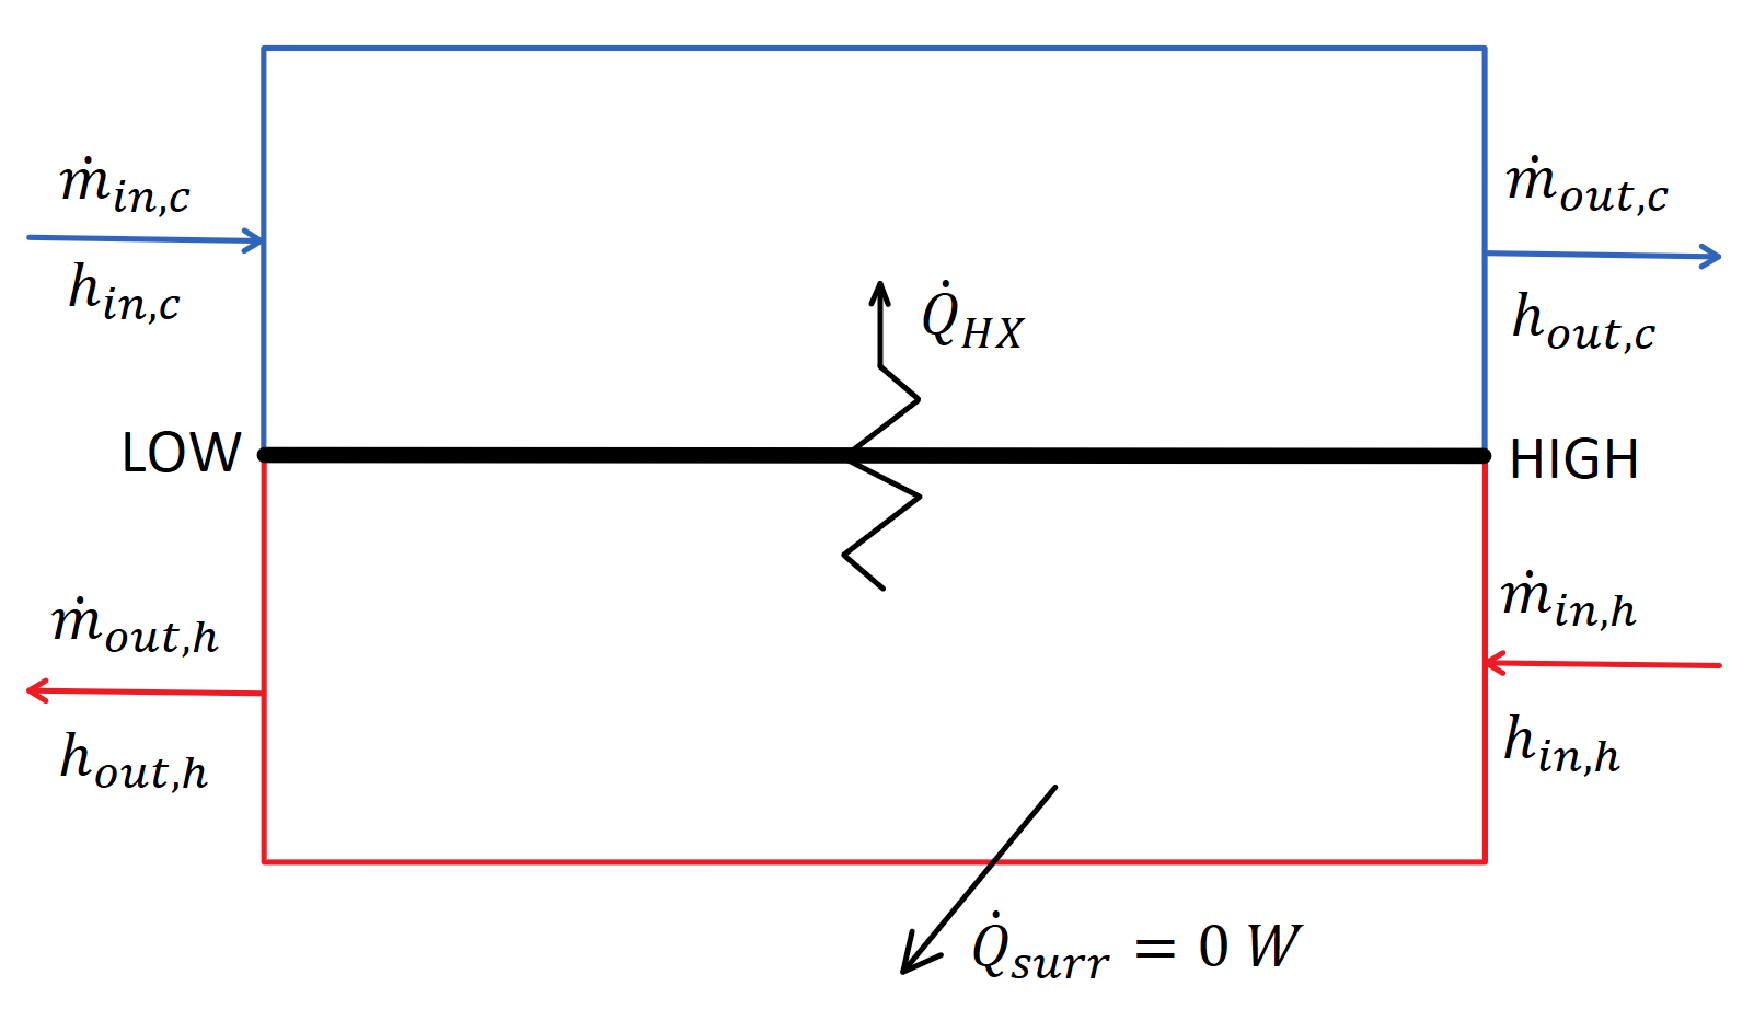
\includegraphics[width=10 cm]{Definitions/counter-flow-hx.pdf}
    \caption{Simple counter flow heat exchanger diagram. \label{counter-flow-hx}}
\end{figure}
\begin{paracol}{2}
\linenumbers
\switchcolumn

Additional assumptions of the counter flow heat exchanger model are: no heat loss to the surroundings, $\dot{Q}_{surr}$ is zero, \mw{these are equivalent} and no pressure drops across the heat exchangers. Counter flow heat exchanger calculations require two known state points, fluid libraries, mass flow rate of hot and cold side, and a specified approach temperature. In all of the modeled cases, the approach temperature is set to a value of $10 K$.\mw{Justify} The fluid libraries referenced are built into EES for Carbon Dioxide and Salt(60\% NaNO3 40\% KNO3) \cite{pacheco_1995_salt_properties,roland_1996_co2_properties}. 

To analyze the counter flow heat exchanger a side is chosen, usually high, to start the calculations. The approach temperature is initially subtracted from the hot stream on the high side to find the missing cold temperature according to Equation \ref{temp_h}. 

\begin{equation}
   \label{temp_h}
    T_{out,c} = T_{in,h}-\Delta_{T},
\end{equation}

Where T$_{out,c}$ is the cold stream outlet temperature and T$_{in,h}$ is the hot stream inlet temperature. Knowing the two state points allows for the enthalpy to be found using correlations from the fluid property libraries. 

[More Desctription on Counterflow HX]

\subsubsection{Lead-Cooled Fast Reactor}
%--------------------------------------------------------------------------------------
Lead-cooled fast reactors use energy from a controlled nuclear reaction to heat molten lead. This lead is used to both cool the core as well as transfer heat into the sCO$_2$ Brayton power cycle \cite{smith_2016_lfr_background,alemberti_2013_lfr_overview}. The lead-cooled fast reactor is assumed to be a black box heat transfer and is labeled in the cycle models LFR HX. The inlet, outlet and heat transfer rates are defined by our industry partner, Westinghouse Electric Company making the black box simplification viable. The energy balance for the black box assumption can be seen in Equation \ref{eq-lfr-black-box}.

\begin{equation}
    \label{eq-lfr-black-box}
    \dot{m}_{inlet}*h_{inlet} + \dot{Q}_{LFRHX} = \dot{m}_{outlet}*h_{outlet},
\end{equation}
\mw{If mass is conserved, use a single $\dot{m}$}

Where the left hand side, $\dot{m}_{inlet}$, $h_{inlet}$, and $\dot{Q}_{LFRHX}$, is the energy into the flow and the right hand side, $\dot{m}_{outlet}$ and $h_{outlet}$, is the energy brought out from the flow of sCO$_2$. The amount of energy transferee into the cycle, $\dot{Q}_{LFRHX}$, is set at $950 MW$, and outlet temperature of the sCO$_2$ from the LFR HX is set at a value of 595$^{\circ}$C. 
\mw{Make sure numbers are in math mode}
The outlet temperature of the LFR is \replaced{specified, accounting for the}{rigid due to} high temperature material limits on the LFR lead side. Low sCO$_2$ LFR inlet temperature has a lower limit of 340$^{\circ}$C and an optimal value of 400$^{\circ}$C.
\mw{How do we know that 400C is the optimal temperature? This information is given to us by Westinghouse, right?} 
Increasing this temperature above this optimal value leads to diminishing returns on the LFR efficiency.


\subsubsection{Concentrating Solar Power Cycle}
%--------------------------------------------------------------------------------------

The CSP salt cycle modeled in this paper is composed of hot and cold thermal energy storage (TES), pumps, receiver, sCO$_2$-to-salt counter flow heat exchanger (C2S), and CSP counter flow heat exchanger (CSP HX). The diagram for this CSP salt cycle is seen in Figure \ref{csp}. 

\mw{Best practice is to allow figures to float. To do this, specify the location as [htb] ("here, top, or bottom"). I've done a search-replace for all figures to do this. }

% \end{paracol}


\begin{figure}[htb] 

    \widefigure
    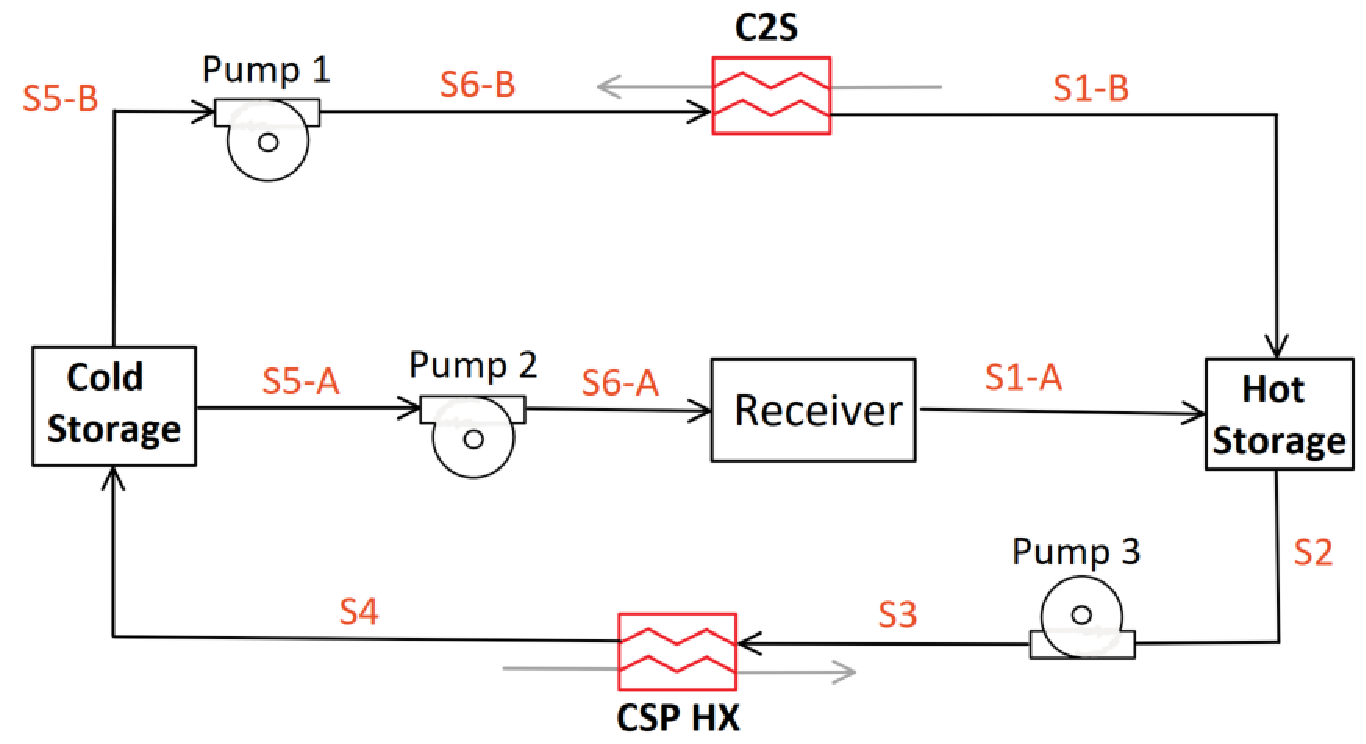
\includegraphics[width=10 cm]{Definitions/csp.pdf}
    \caption{Diagram for CSP cycle with cold and hot thermal energy storage, pumps, and csp black box heat input\label{csp}}
\end{figure}
% \begin{paracol}{2}
% \linenumbers
% \switchcolumn

The CSP salt cycle uses 60\% sodium nitrate and 40\% potassium nitrate 'solar salt' as the heat transfer fluid. Solar salt stored in the hot TES can be dispatched on demand through the CSP HX when grid demand increases and held when grid demand is low. Current CSP salt cycles heat solar salt with receivers and store it in hot TES tanks at 565$^{\circ}$C. Future CSP salt cycles are hypothesized to have bulk hot TES temperatures of up to 720$^{\circ}$C, but due to high temperature limitations with the LFR outlet, the hot TES temperature is set at 595$^{\circ}$C for all modeled cycles \cite{mehos2017concentrating}. The cold TES temperature takes on three different values according to cycle configuration capabilities: 390$^{\circ}$C, 410$^{\circ}$C, and 440$^{\circ}$C. In addition to the lower hot TES temperature, current CSP salt cycles lack a secondary option for charging the hot TES \cite{hamilton2020dispatch}. The studied CSP salt cycle has two TES charging options: a receiver, which generates heat from a heliostat field, and C2S heat exchanger, which draws excess heat from the sCO$_2$ Brayton cycle. It is assumed that only one hot TES charging option can be active at any given time. 

The C2S heat exchanger is active \replaced{in}{during} the 'charging' cycle configurations, when the focus is on heat storage for later use. During this process there is no solar salt flow through the receiver. \mw{Is this necessarily true? Couldn't there be a condition where we'd like to dump energy from the LFR while simultaneously collecting from CSP?} Pump 1 is actively moving solar salt from cold TES to hot TES through the C2S heat exchanger, which is extracting heat from the sCO$_2$ Brayton cycle. 

'Non-charging' cycle configurations \replaced{are characterized by operations wherein}{has} the receiver is charging the hot TES, the C2S heat exchanger is not transferring heat, and the LFR is \replaced{heat}{dispatching energy} directly to generate electricity. When electrical generation is occurring, the heat input in this \mw{``this'' is ambiguous} cycle is modelled through a black box energy balance across states S6-A and S1-A with a heat addition of 7.5e8 W from the heliostat field. The hot storage is moved through Pump 3 and transfers heat into the sCO$_{2}$ Brayton cycle to be converted into electricity. The cooled salt is stored in cold storage and moved through Pump 2 where the heat addition from the receiver is added.



\subsection{Generalization of Cycle Modeling}
%======================================================================================
\mw{What do you mean by ``generalized?''}

\mw{We need an overview here of our process for identifying which cycles will be modeled, as the discussion below gets a bit complicated with all of the different permutations. It might be helpful to have a model taxonomy that schematically shows how the different models are related to each other.}

\replaced{In order to draw a more direct comparison, the cycles are generalized in terms of}{The cycles presented are generalized in order to draw a more direct comparison. The generalized parameters include} isentropic efficiencies, heat exchanger approach temperatures, pressures, heat input, and pump constants. These values are summarized in Table \ref{tab-cycle-constants}.

\begin{specialtable}[htbp] 
    \mw{Also changing the specialtable position to allow latex to better place tables.}

    \caption{Constant cycle parameters with definition, variable and set value. \label{tab-cycle-constants}}
    \begin{tabular}{L{0.5\linewidth}cc}
    \toprule
    \textbf{Parameter} & \textbf{Variable}	& \textbf{Design Point Value}\\
    \midrule
    \textit{Efficiencies}\\
    Main Compressor & $\eta_{MC}$		& 0.91 (-)\\
    Re-Compressor & $\eta_{RC}$		& 0.89 (-)\\
    Turbine & $\eta_{T}$		& 0.90 (-)\\
    Pump & $\eta_{P}$      & 0.90 (-)\\
    \midrule
    \textit{Approach Temperatures}\\
    Low Temperature Recuperator & $\delta_{LTR}$		& 10 (K)\\
    High Temperature Recuperator & $\delta_{HTR}$		& 10 (K)\\
    Concentrating Solar Power Heat Exchanger & $\delta_{CSPHX}$	& 10 (K)\\
    \midrule
    \textit{Pressures}\\
    Pressure Ratio & $PR$ & 3.27 (-)\\
    High Side Pressure & $P_{2A}$ & 2.88e7 (Pa)\\
    \midrule
    \textit{Heat Into System}\\
    Lead-Cooled Fast Reactor Heat Transfer & $\dot{Q}_{LFRHX}$ & 9.5e8 (W)\\
    Concentrating Solar Power Heat Transfer & $\dot{Q}_{CSP}$ & 7.5e8 (W)\\
    \midrule
    \textit{Temperature}\\
    Main Compressor Inlet & $T_{1A}$ & 313.2 (K)\\
    %Lead-Cooled Fast Reactor sCO$_{2}$ Low Temperature & $T_{4}$,$T_{1C}$,$T_{5A}$,$T_{4C}$ & 673.2 (K)\\
    Lead-Cooled Fast Reactor sCO$_{2}$ High Temperature & $T_{5}$,$T_{2C}$,$T_{6A}$,$T_{5C}$ & 868.2 (K)\\
    \midrule
    \textit{Pumps}\\
    Pressure Rise Across Pump & $\Delta_{P}$ & 3.726e6 (Pa)\\
    Pump Low Side Pressure & $P_{S5-B}$ & 3.0e6 (Pa)\\ 
    \bottomrule
    \end{tabular}
\end{specialtable}

The values displayed in Table \ref{tab-cycle-constants} are representative of LFR and CSP design while being consistent with design parameters given by our industry partner, Westinghouse Electric Company. 

In addition to generalized parameters, all cycles have identical recompression sides. The recompression side contains a PreCooler, Low Temperature Recuperator, and two compressors; Main Compressor and ReCompressor. \mw{components don't need to be capitalized -- they aren't proper nouns}

Modeled cycles are summarized in Table \ref{tab-cycle_sum}.

\begin{specialtable}[H] 
    \caption{Summary of all modeled non-charging and charging cycles with descriptions. \label{tab-cycle_sum}}
    \begin{tabular}{lL{0.7\linewidth}}
    \toprule
    \textbf{Cycle Label} & \textbf{Description}\\
    \midrule
    \textit{Non-Charging}\\
    C-LFR-ON & Two-cycle configuration with LFR as heat source.\\
    C-CSP-ON & Two-cycle configuration with CSP as heat source.\\
    C-1HTR1T-ON & CSP and LFR heat sources in parallel with one turbine.\\
    C-2HTR3T-ON & Seperatre CSP and LFR loops each with dedicated HTR and turbine.\\
    \midrule
    \textit{Charging}\\
    C-LFR-PRE & Turbine is prior to the SALT HX.\\
    C-LFR-POST & Turbine is after the SALT HX.\\
    C-LFR-PAR & Turbine is parallel to the SALT HX.\\
    C-LFR-CIRC & Circulator bridges the LFR and SALT HX.\\
    \bottomrule
    \end{tabular}
\end{specialtable}

\subsection{Non-Charging Cycle Configurations} 
%======================================================================================

Various cycles are modeled to test their advantages and disadvantages. These cycle models fall into two categories: non-charging and charging. The non-charging category is used to determine the configuration of the cycle with a focus on electricity generation. This includes the number and location of turbines, recuperators, and heat input to the system by the CSP and LFR. To quantify the effectiveness of the non-charging configurations, a cycle efficiency, $\eta_{cycle}$, is defined in Equation \ref{eq-eta-cycle}.

\begin{equation}
    \label{eq-eta-cycle}
    \eta_{cycle} = \frac{\dot{W}_{T}-\dot{W}_{MC}-\dot{W}_{RC}}{\dot{Q}_{LFRHX}+\dot{Q}_{CSPHX}},
\end{equation}

The numerator in Equation \ref{eq-eta-cycle} is the \replaced{alternator}{Alternator} power, or the power produced from the turbines, $\dot{W}_{T}$, minus the required power of the compressors, $\dot{W}_{MC}$ and $\dot{W}_{RC}$. The denominator is the total power input into the system from the LFR HX, $\dot{Q}_{LFRHX}$, and CSP HX, $\dot{Q}_{CSPHX}$.


\subsubsection{Two-Cycle Configuration: C-LFR-ON and C-CSP-ON} %--------------------------------------------------------------------------------------

The two-cycle configuration that is tested has independent sCO$_{2}$ loops \replaced{that share a common}{bridged by a} CSP cycle. This cycle has two sCO$_{2}$ Brayton Cycles: C-LFR-ON and C-CSP-ON. Configuration of components for these two cycles is identical with the exception of heat inputs. C-LFR-ON has heat provided from a LFR while C-CSP-ON has heat provided from the CSP. These two cycles individually operate when the focus of plant operation is primarily electricity generation.

The cycle that is using the LFR heat input in the two-cycle configuration is labeled as C-LFR-ON and the cycle diagram is illustrated in Figure \ref{c-lfr-on}. \mw{There are lots of little 1-2 sentence ``paragraphs'' that could be consolidated with some thought.}

\end{paracol}
\begin{figure}[!h] 
    \widefigure
    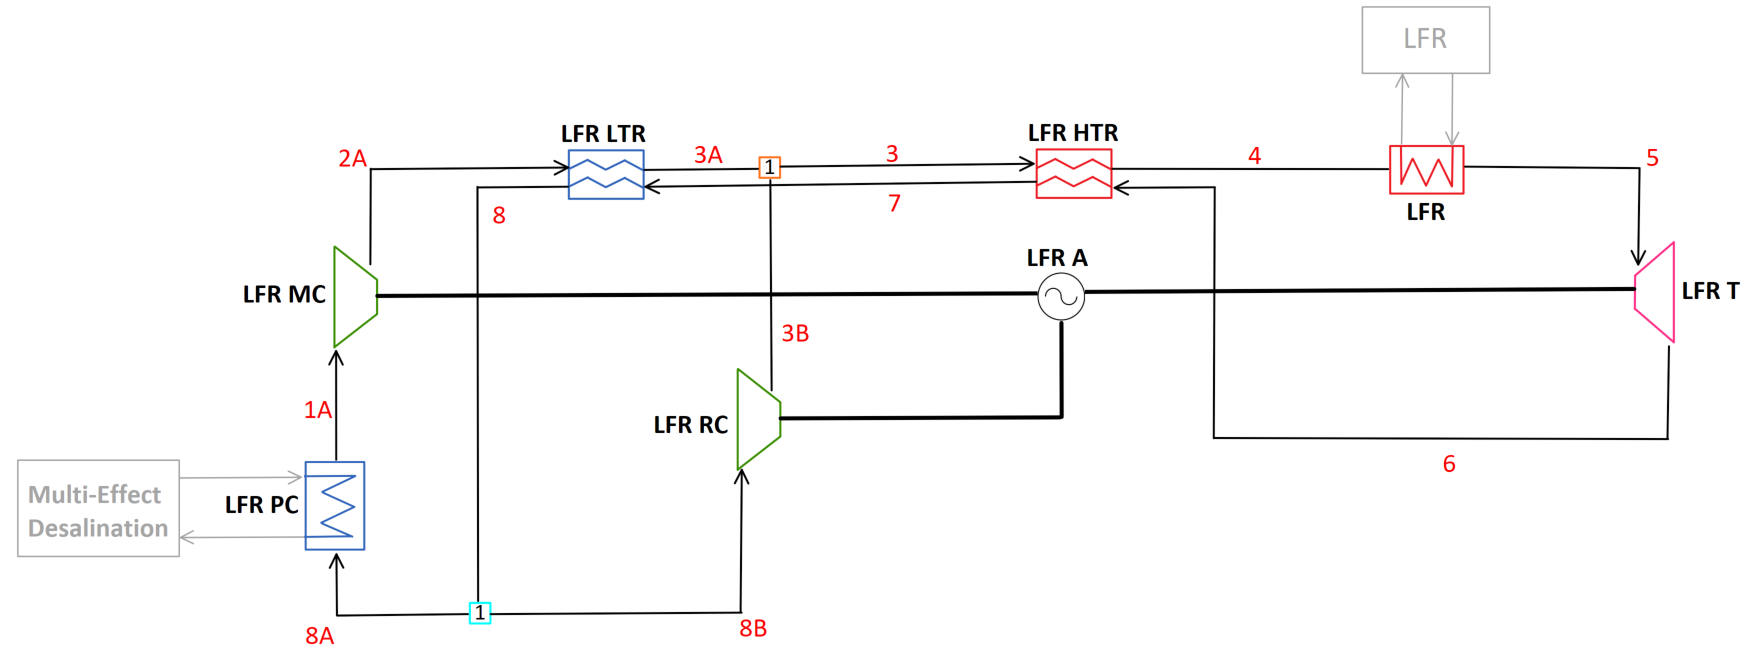
\includegraphics[width=\linewidth]{Definitions/c-lfr-on.pdf}
    \caption{Diagram for C-LFR-ON with focus on electricity generation\label{c-lfr-on}}
\end{figure}
\begin{paracol}{2}
\linenumbers
\switchcolumn

Two separate sensitivity studies on the LFR inlet temperature are completed for C-LFR-ON. The unconstrained study is performed by gradually increasing the mass flow to the main compressor while maximizing cycle efficiency. The constrained study is calculated by setting the LFR inlet temperature to the design value of 673.2 K (400$^{\circ}$C), which is a requirement of the LFR primary circuit to maximize power output within material limits.
\bl{flip the order of this para: constrained then unconstrained. State that the unconstrained is a 'sensitivty' case to determine the penalty of the constraint}
% 
The cycle that is using the CSP heat input in the two-cycle configuration is labeled C-CSP-ON and the cycle diagram is shown in Figure \ref{c-csp-on}. 

\end{paracol}
\begin{figure}[!h] 
    \widefigure
    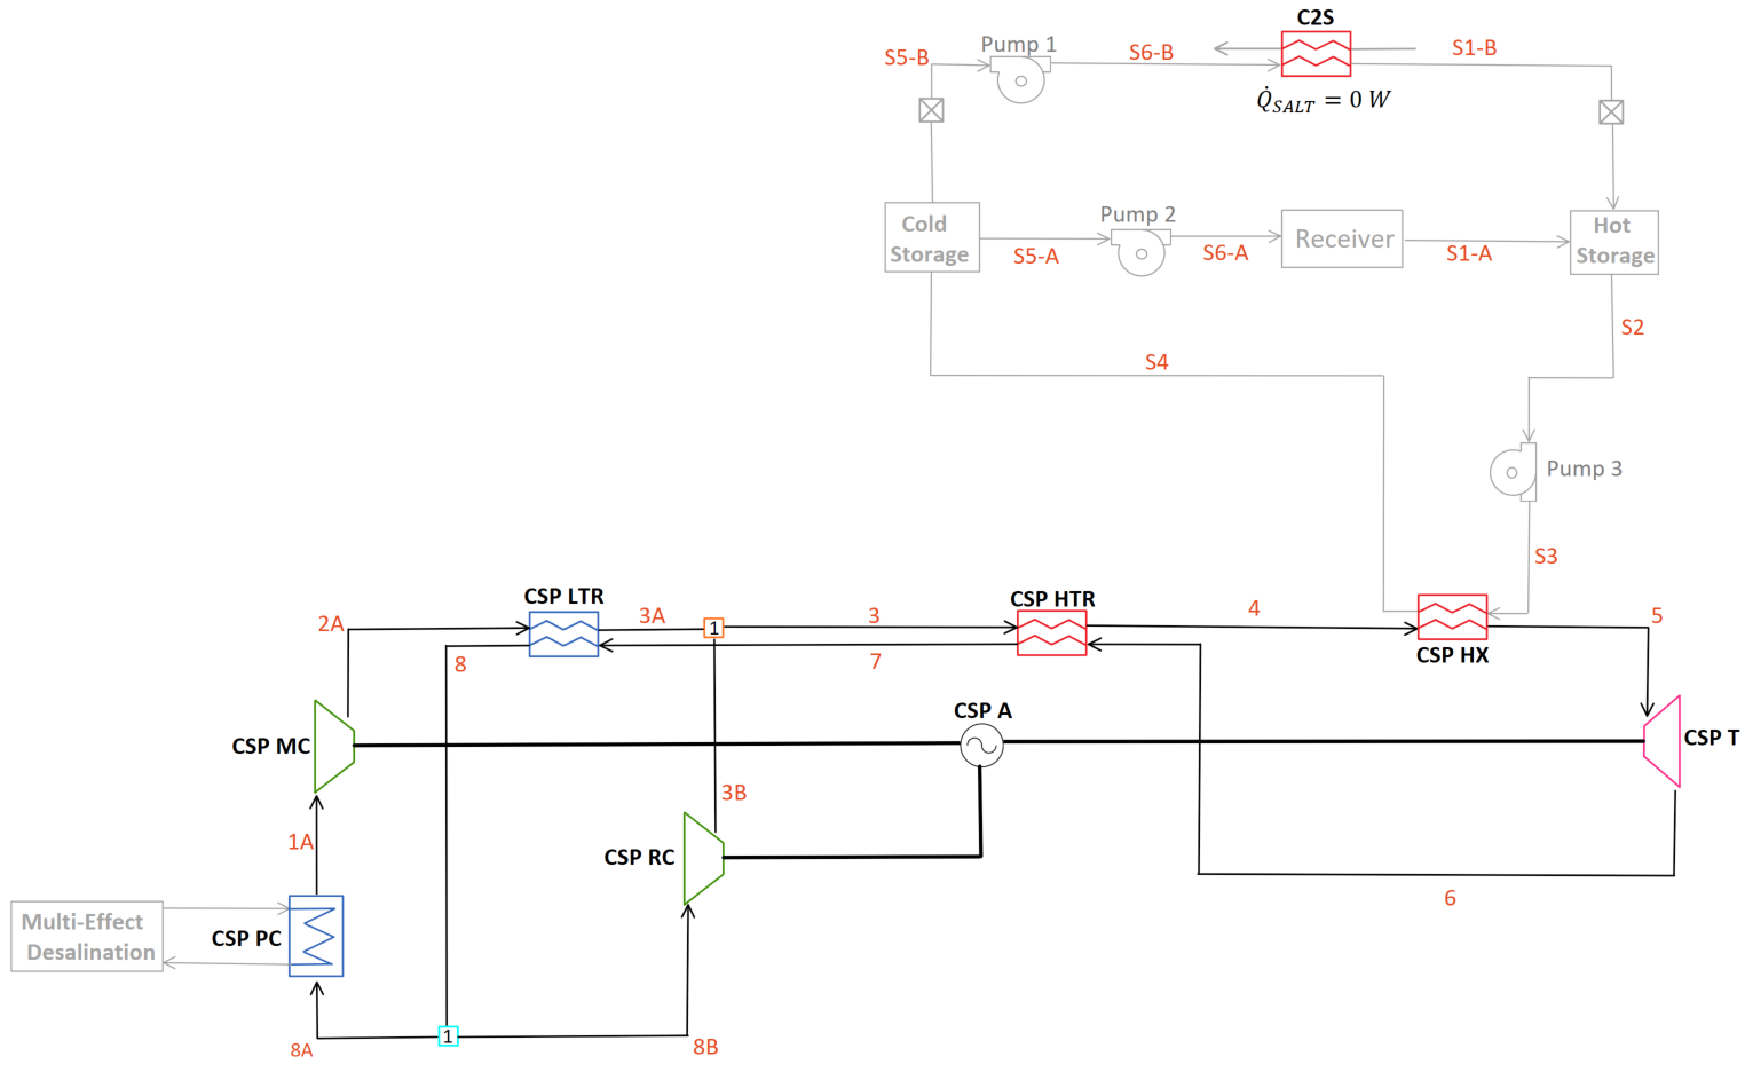
\includegraphics[width=\linewidth]{Definitions/c-csp-on.pdf}
    \caption{Diagram for C-CSP-ON with focus on electricity generation\label{c-csp-on}}
\end{figure}
\begin{paracol}{2}
\linenumbers
\switchcolumn

 Due to the individual operation while the cycles are generating electricity, C-CSP-ON is not directly impacted by the LFR low end temperatures. Instead, a sensitivity study is done on the temperature of the cold TES. Two temperatures are tested, 663.2 K and 713.2 K, to observe the impact of cold TES temperature on cycle efficiency. 


\subsubsection{C-1HTR1T-ON} 
%--------------------------------------------------------------------------------------

One drawback of having a two-cycle design, as seen in the C-LFR-ON and C-CSP-ON, is doubling the number of system components. Combining the two cycles into one would reduce redundancy and complexity. Heat addition from the CSP HX and LFR HX in parallel orientation is therefore studied in the C-1HTR1T-ON model. This model studies what impact mixing different temperature flows prior to the turbine has on cycle efficiency. The diagram for this cycle is illustrated in Figure \ref{c-1htr1t-on}.

\bl{be clear that Salt HX links back into the sCO2 cycle (e.g. parallel to 5-6) but is not shown to simplify the diagram. Otherwise people will wonder where it is coming from}
\mw{After lots of tinkering, I've not solved how to get the figures to avoid spilling over the edge of the page. I think it's a problem with the MDPI template. The figures have a lot of whitespace between components and numbers, and you may need to try to compress some of them down to make them more compact.}
\end{paracol}

\begin{figure}[H] 
    \widefigure
    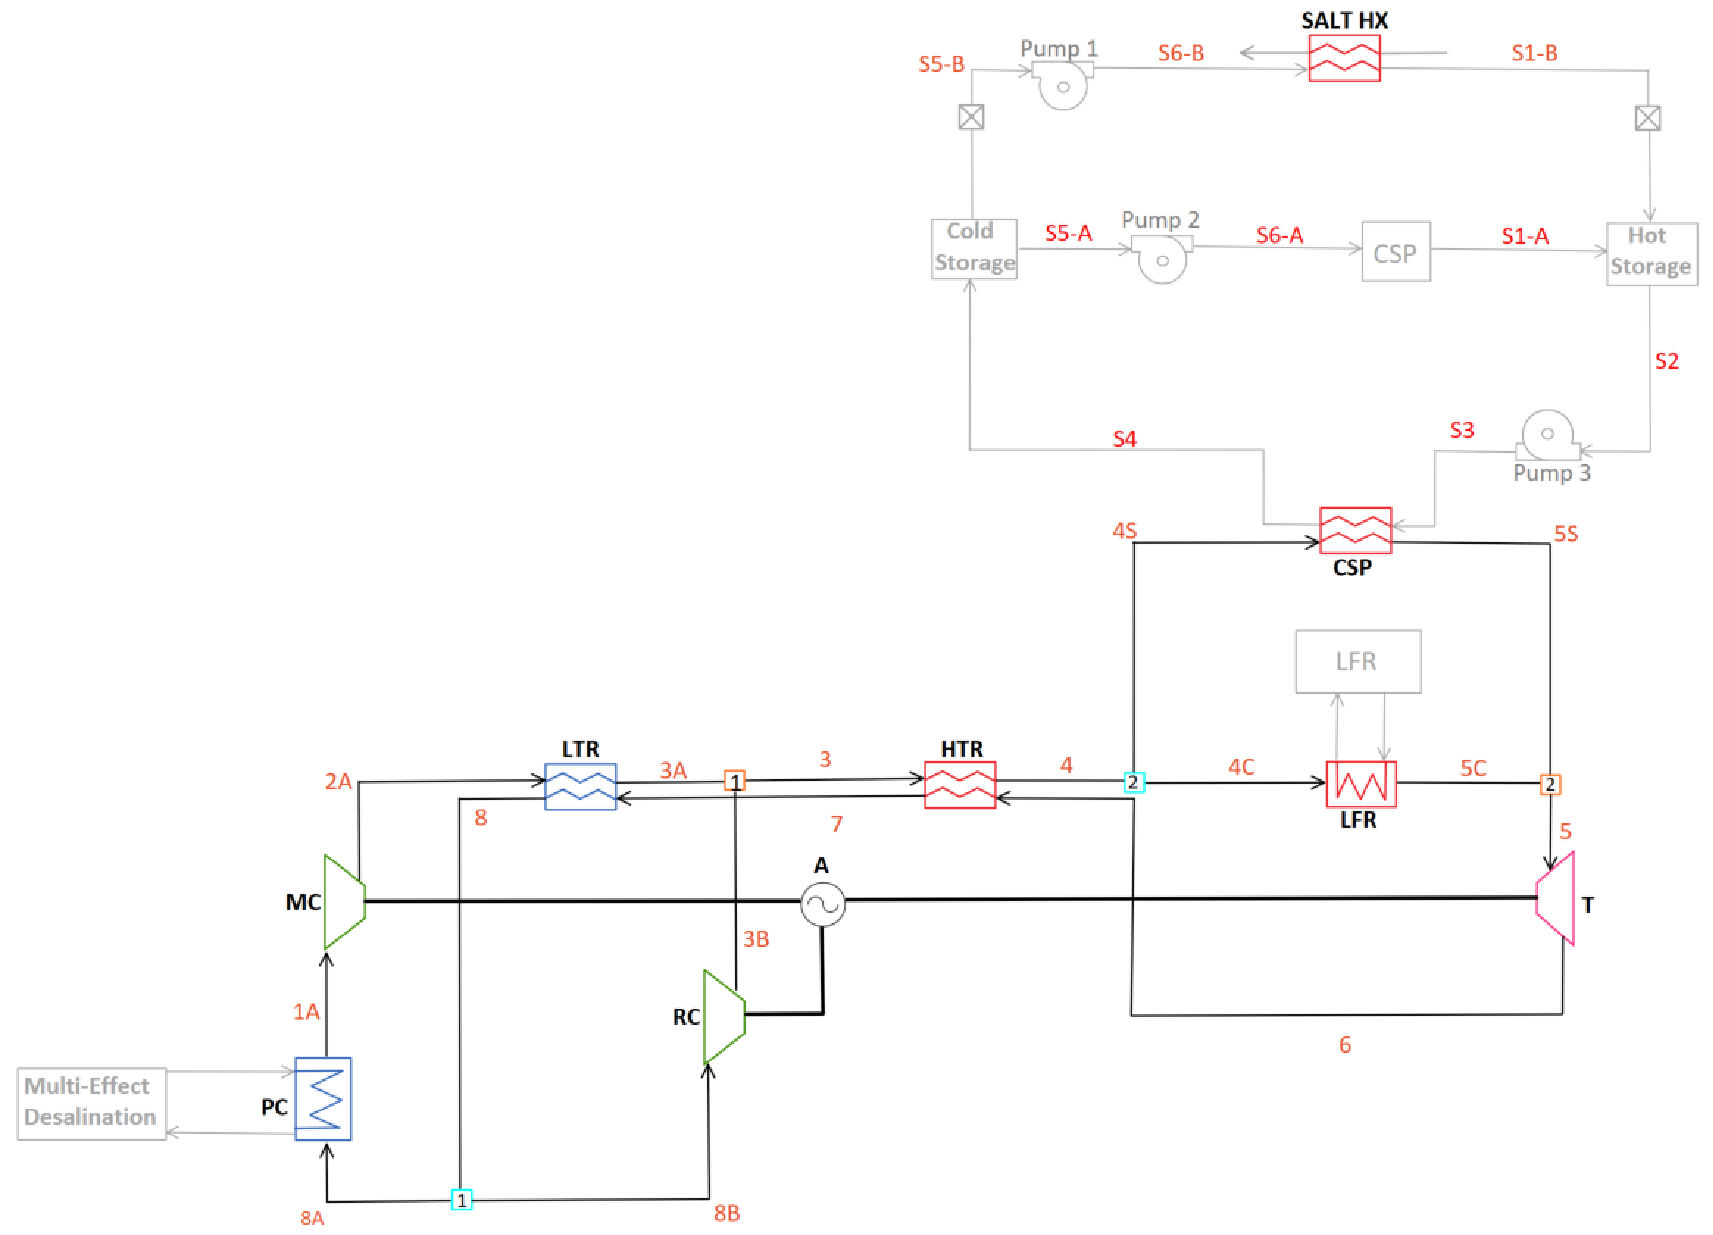
\includegraphics[width=\linewidth]{Definitions/c-1htr1t-on.pdf}
    \caption{Diagram for C-1HTR1T-ON with focus on electricity generation\label{c-1htr1t-on}}
\end{figure}


\begin{paracol}{2}
\linenumbers
\switchcolumn

In this cycle, the LFR HX and CSP HX have identical inlet temperatures due to splitting the flow prior to their parallel orientation. Therefore, three sensitivity studies are done on the C-1HTR1T-ON EES model. The initial two studies have the low LFR temperature constrained to the value of 673.2 K with varied cold CSP TES \mw{varied cold CSP TES ... what? temperature?} and maximized cycle efficiency. \mw{State what variable(s) are manipulated in order to maximize cycle efficiency} \replaced{Two cold CSP TES temperature values are tested (683.2 K and 713.2 K)}{The two tested values for cold CSP TES} with constrained LFR low temperature\deleted{ are 683.2 K and 713.2 K}. The desired cold CSP TES temperature of 663.2 K is not possible with the constraint on the LFR low temperature (because it cannot be colder than the sCO$_2$ that removes heat from the salt). In this case, to obtain the desired cold CSP TES temperature, the constraint on the LFR low temperature is removed, dropping the temperature of the LFR inlet to 653.2 K. 
\bl{I think I understand what you're talking about but the above para could spell out all the sensitivity cases a bit more clearly, perhaps as bullets. Asp you will want to explain the criteria that go into cold storage temp. Lower = more delta T = more dispatchability}


\subsubsection{C-2HTR3T-ON} 
%--------------------------------------------------------------------------------------

Mixing two different temperature flows before the turbine in a Brayton cycle has a negative effect on cycle efficiency \mw{compared to...?}. To quantify the reduction in cycle efficiency, another cycle with no mixing prior to the turbine is desired. This cycle, C-2HTR3T-ON, can be seen in Figure \ref{c-2htr3t-on} and has two high temperature recuperators and three turbines. The LFR is powering one turbine, T1, and recuperating heat through a dedicated high temperature recuperator, HTR1. \mw{The LFR doesn't recuperate heat. Clarify what you mean here.} The CSP cycle \mw{CSP cycle refers to the salt loop. Here we mean something else.} also contains two separate turbines, T2, while having a dedicated high temperature recuperator, HTR2. \mw{Need to explain how T2 is actually 2 separate turbines represented diagramatically as 1, and why we can model it this way.} After the high temperature recuperators, the two flows are combined and sent to the LTR hot side. 
\bl{this is more about having a compromise option of intermediate complexity and efficiency}

\end{paracol}
\begin{figure}[H]
    \widefigure
    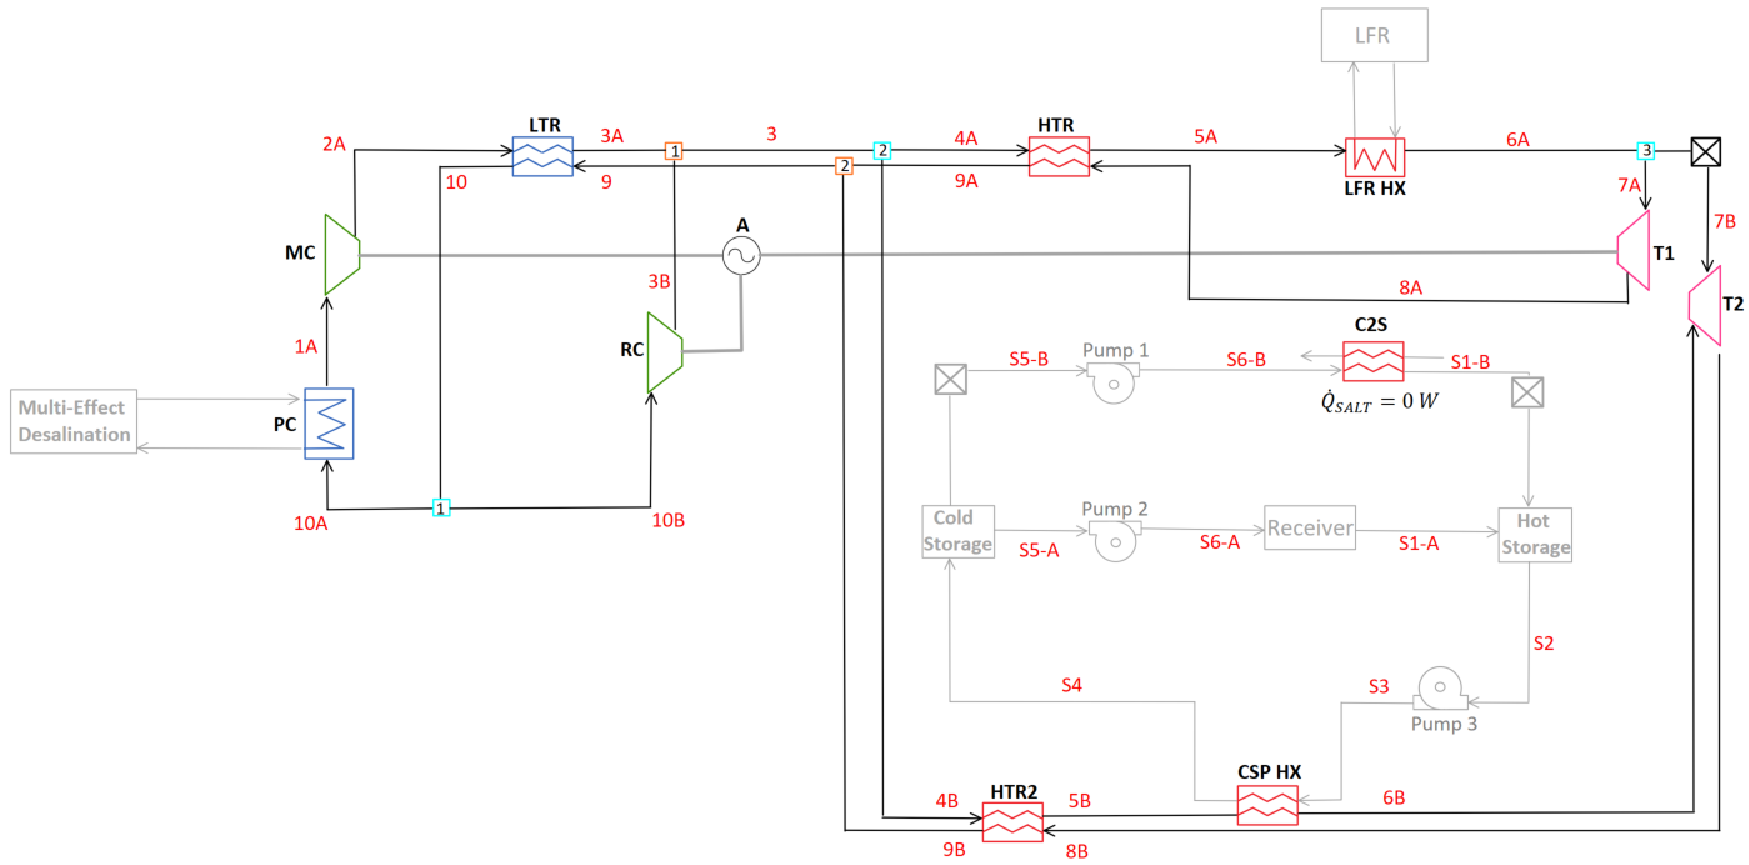
\includegraphics[width=\linewidth]{Definitions/c-2htr3t-on.pdf}
    \caption{Diagram for C-2HTR3T-ON with focus on electricity generation\label{c-2htr3t-on}}
\end{figure}
\begin{paracol}{2}
\linenumbers
\switchcolumn

Three sensitivity studies are done on the C-2HTR3T-ON model -- two with the LFR low temperature constrained and one without this constraint. The two constrained studies had varied\mw{present tense} cold CSP TES temperature with the lowest temperature of 663.2 K and highest temperature of 713.2 K. The unconstrained low LFR inlet study is calculated at a cold CSP TES temperature of 663.2 K.  
\bl{this is clearer than the previous one but bullets could still be useful}



\subsection{Thermal Energy Storage Charging Techniques} 
%======================================================================================

Charging cycle configurations \replaced{accommodate}{focus on an} energy storage \replaced{modes of operation}{operating mode}. These configurations \replaced{examine the}{test the optimal} location of LFR heat extraction \replaced{via}{through} the SALT HX. To maximize the available heat for extraction, alternator \added{net} power is set to zero\added{, therefore requiring that the} turbine power is \deleted{therefore} equal to the compressors' demand. The excess energy from the LFR is thermally stored in the TES for later use when grid demand increases. \replaced{The location of heat extraction}{Comparison of where thermal energy is extracted} in the cycle is \replaced{compared within the C-LFR-ON Brayton cycle by placing}{done by using the same Brayton cycle, C-LFR-ON, and configuring} the salt heat exchanger in different locations around the turbine. To quantify the effectiveness of TES charging techniques a heat storage efficiency, \added{we define the metric} $\eta_{heatstorage}$ \deleted{, is defined by} in Equation \ref{eq-eta-heatstorage}.
\bl{explain that as a (re)compression cycle is still being run for the LFR and the components are not perfectly efficient, it will consume power moving the fluid around that needs to be balanced with some of the thermal output}

\begin{equation}
    \label{eq-eta-heatstorage}
    \eta_{heatstorage} = \frac{\dot{Q}_{C2S}}{\dot{Q}_{LFRHX}+\dot{Q}_{CSPHX}},
\end{equation}

Whereas $\dot{Q}_{S2C}$ is the amount of heat transferred through S2C and the addition of $\dot{Q}_{LFRHX}$ and $\dot{Q}_{CSPHX}$ is the total amount of heat input into the system from the LFR HX and CSP HX. \mw{not a full sentence}

\subsubsection{C-LFR-PRE} 
%--------------------------------------------------------------------------------------

Flow leaving the turbine contains excess thermal energy that is not transformed into electrical energy. This excess thermal energy is stored in the hot CSP TES. \mw{Careful here. Be precise about what ``excess'' means in this context. Any fluid above absolute zero technically has excess thermal energy if the reference is zero. Depending on this definition, not all excess energy from the turbine is stored in TES.} The diagram outlining this process is C-LFR-PRE in Fig. \ref{c-lfr-pre}.  \mw{explain in a bit more detail what is happening that makes this configuration different from prior iterations.}

\end{paracol}
\begin{figure}[H]
    \widefigure
    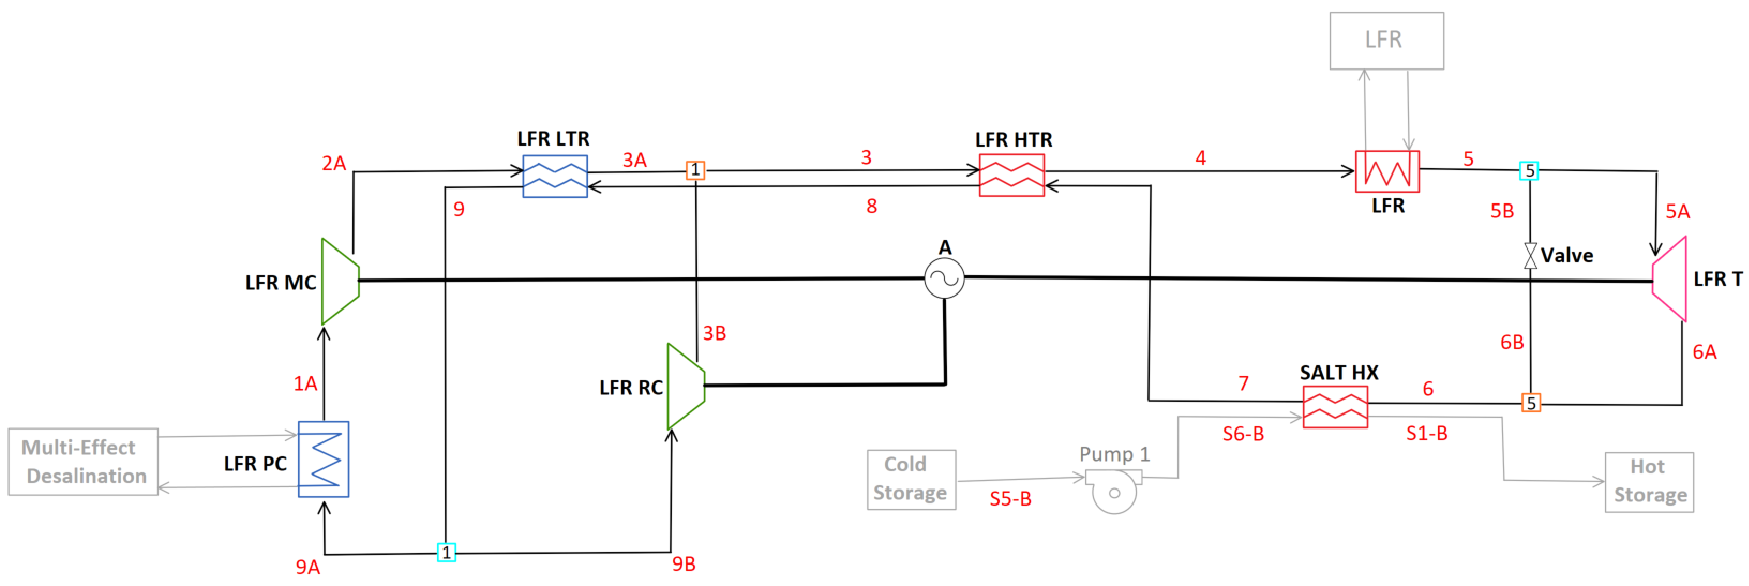
\includegraphics[width=\linewidth]{Definitions/c-lfr-pre.pdf}
    \caption{Diagram for C-LFR-PRE thermal energy storage charging orientation\label{c-lfr-pre}}
\end{figure}
\begin{paracol}{2}
\linenumbers
\switchcolumn

Problems arise with this salt charging configuration. The temperature out of the turbine is not high enough to charge the hot CSP TES to the required value of 833.2 K. To raise the temperature, some of the high temperature flow before the turbine is redirected through a valve and combined after the turbine. Combining different temperature flows and reducing the flow through the turbine has a large impact on heat storage efficiency. 



\subsubsection{C-LFR-POST} 
%--------------------------------------------------------------------------------------

Moving the heat extraction prior to the turbine is analyzed in C-LFR-POST. This diagram is seen in Figure \ref{c-lfr-post}.

\end{paracol}
\begin{figure}[H]
    \widefigure
    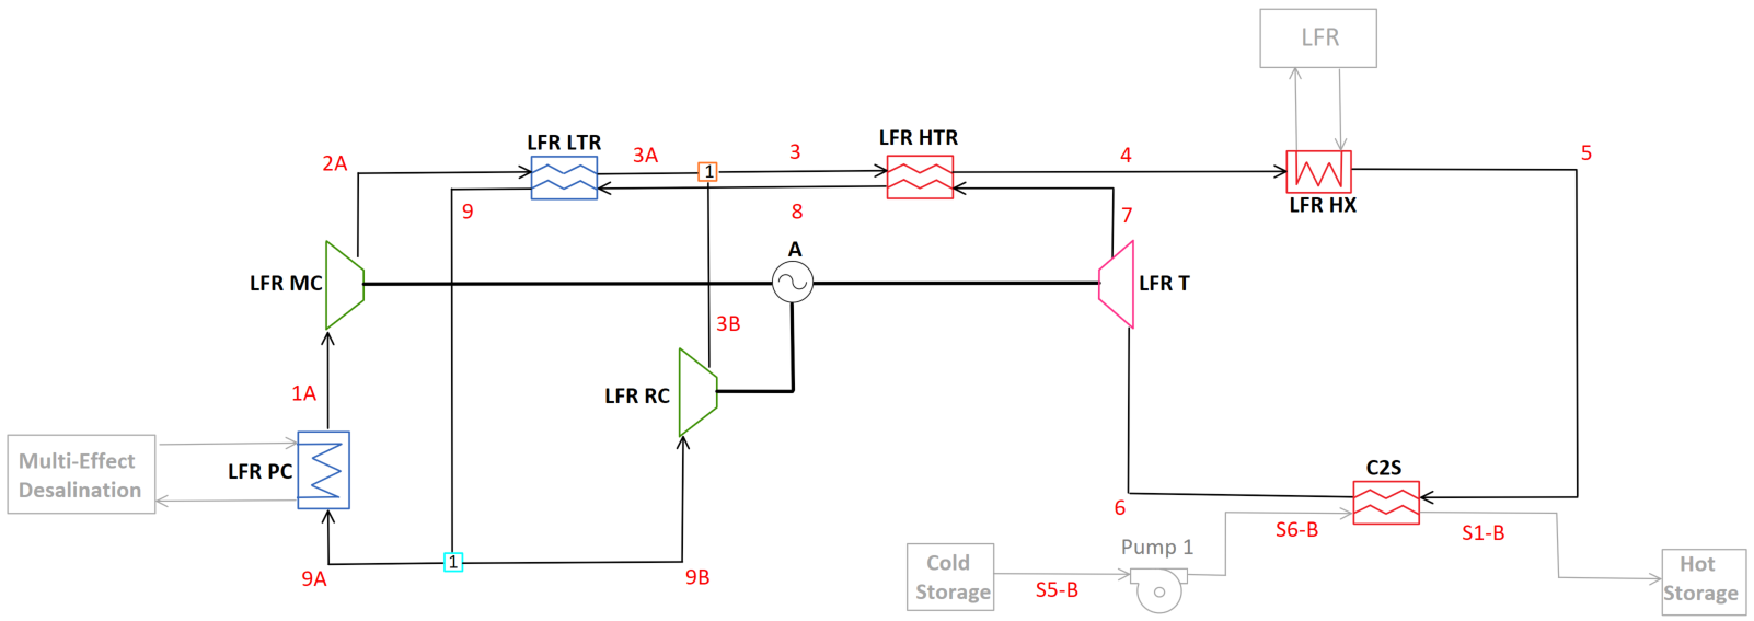
\includegraphics[width=\linewidth]{Definitions/c-lfr-post.pdf}
    \caption{Diagram for C-LFR-POST thermal energy storage charging orientation\label{c-lfr-post}}
\end{figure}
\begin{paracol}{2}
\linenumbers
\switchcolumn

This TES charging cycle extracts heat before the turbine and therefore would have \mw{tense.. it ``has''} a large negative effect on the amount of work that the turbine could \mw{tense} produce. The turbine needs to offset \mw{the turbine does not have feelings :)} the requirements of both compressors and this would require the inlet temperature to be high. The amount of energy that could be extracted before the turbine would be small and therefore the heat storage efficiency would be small. There is no quantitative study done on this case because, due to the efficiency losses, it is non-viable. \mw{write matter-of-factly, not in a hypothetical tense.}

\subsubsection{C-LFR-PAR} 
%--------------------------------------------------------------------------------------

The requirements of the turbine and CSP hot TES can be \replaced{satisfied}{accomplished} by splitting the flow before the turbine. The flow through the salt heat exchanger in this cycle is therefore separate from the turbine. After the salt heat exchanger, a valve is needed to reduce the pressure, this TES charging cycle is C-LFR-PAR shown in Figure \ref{c-lfr-par}.

\end{paracol}
\begin{figure}[H]
    \widefigure
    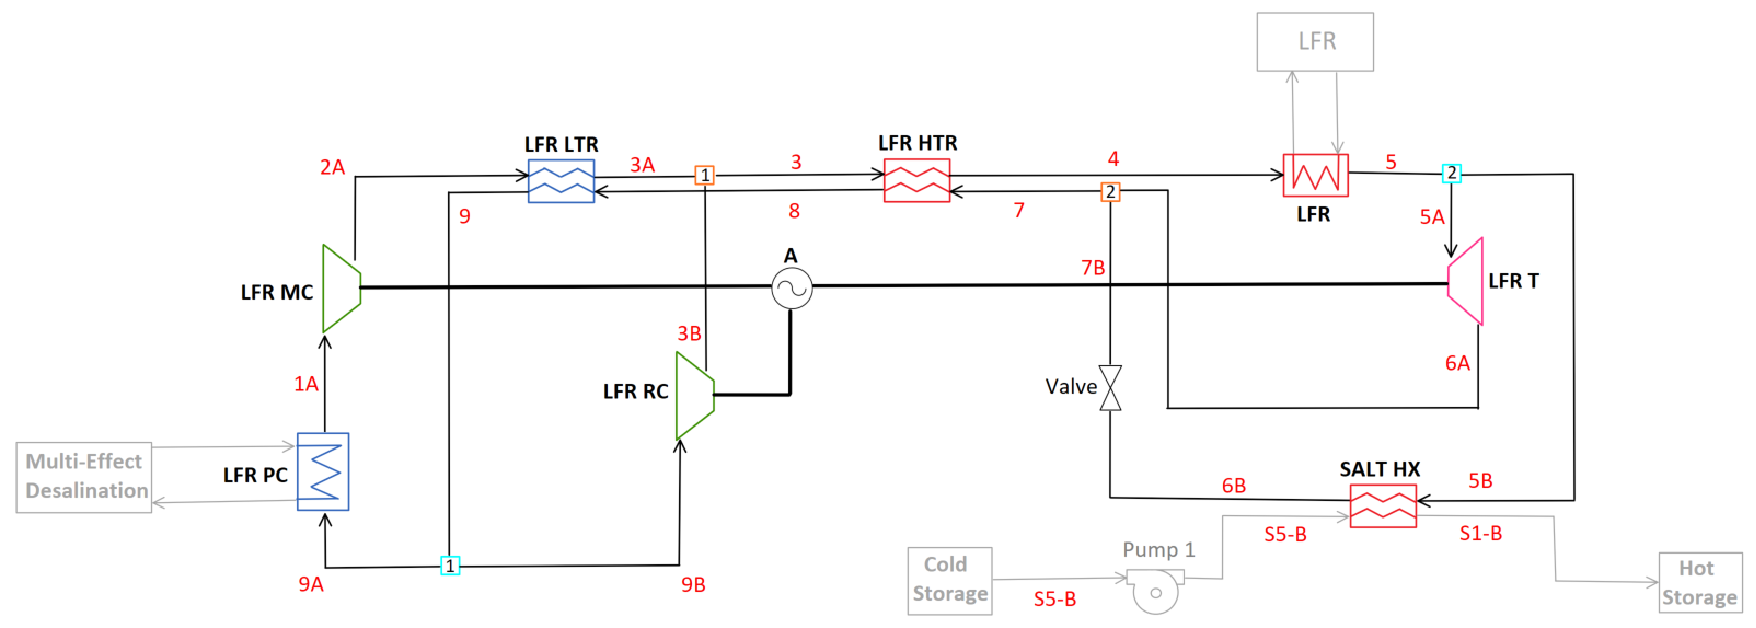
\includegraphics[width=\linewidth]{Definitions/c-lfr-par.pdf}
    \caption{Diagram for C-LFR-PAR thermal energy storage charging orientation\label{c-lfr-par}}
\end{figure}
\begin{paracol}{2}
\linenumbers
\switchcolumn

Two sensitivity studies \mw{this is one study with two parameter values, right?} with varying cold CSP TES \added{temperature} are \replaced{carried out to determine}{desired to see} the impact on heat storage efficiency. \replaced{The study considers two temperature values of 663.2 K and 713.2 K.}{The TES temperature study is calculated with a low TES temperature of 663.2 K and a high TES temperature of 713.2 K.} \mw{make sure I didn't change the meaning here}

\subsubsection{C-LFR-CIRC} 
%--------------------------------------------------------------------------------------

The full diagram for C-LFR-CIRC is shown in Figure \ref{c-lfr-circ}.

\end{paracol}
\begin{figure}[H]
    \widefigure
    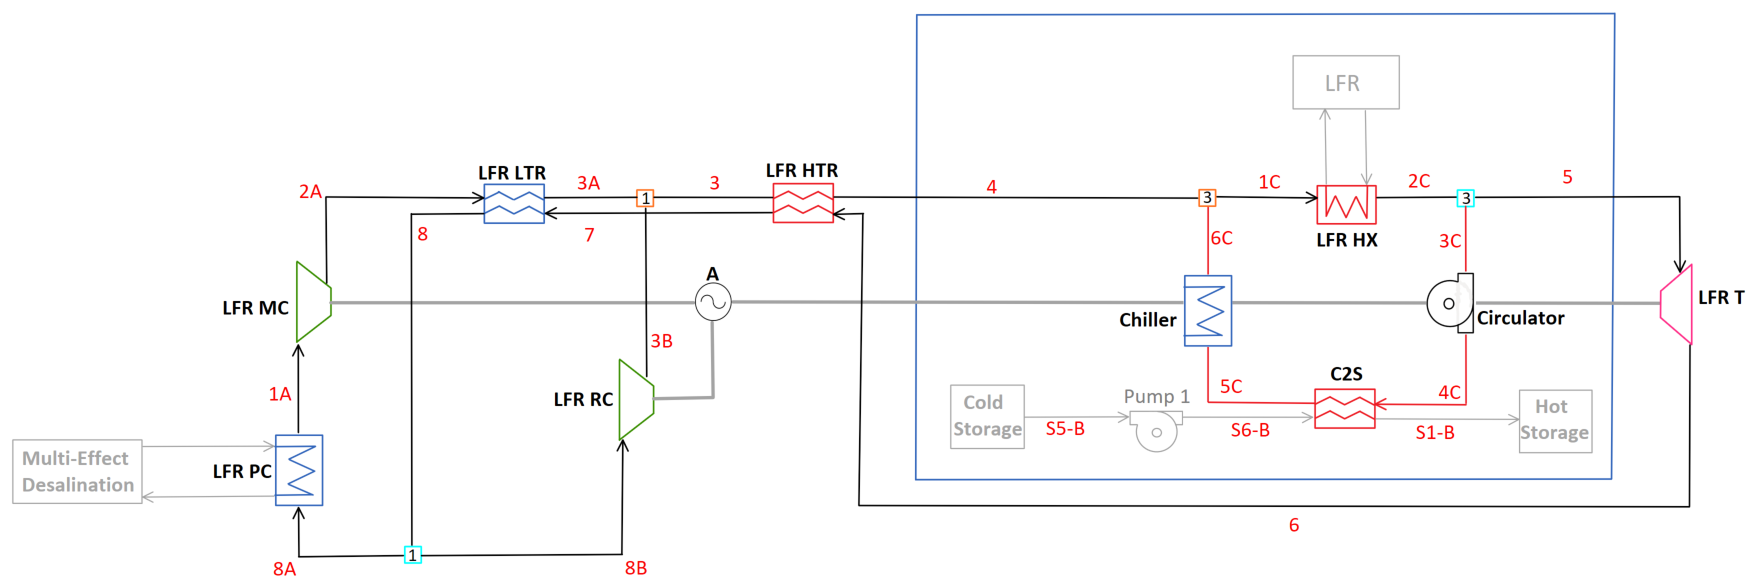
\includegraphics[width=\linewidth]{Definitions/c-lfr-circ.pdf}
    \caption{Full diagram for C-LFR-CIRC thermal energy storage charging orientation\label{c-lfr-circ}}
\end{figure}
\begin{paracol}{2}
\linenumbers
\switchcolumn

The charging subsection of this diagram is composed of a circulation cycle that has heat inputted through the LFR heat exchanger. This subsection is encircled in blue and can be seen in Figure \ref{c-lfr-circ-sub}.

\bl{explain why you are considering this case (avoid losing useful energy in compressor and turbine inefficiencies)} \mw{agree with Ben. Additional motivation is needed}

\end{paracol}
\begin{figure}[H]
    \widefigure
    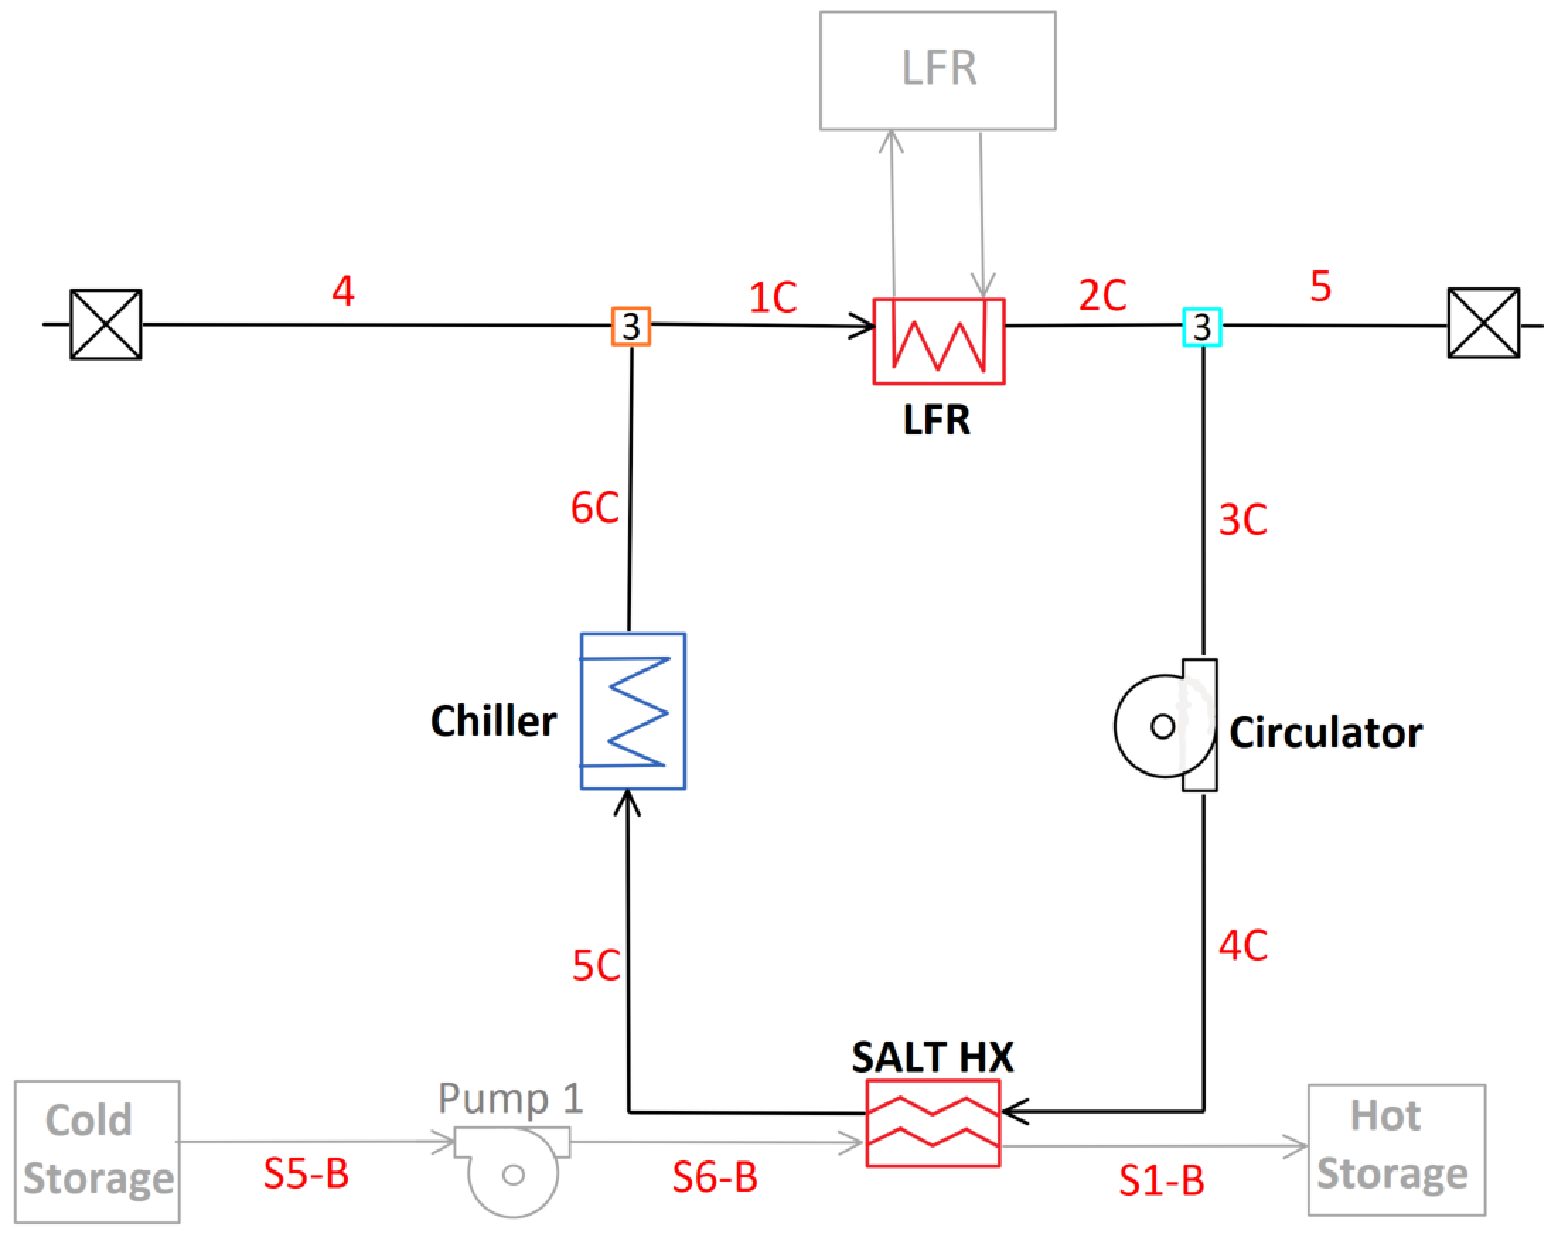
\includegraphics[width=10 cm]{Definitions/c-lfr-circ-sub.pdf}
    \caption{Diagram for C-LFR-CIRC sub-cycle thermal energy storage charging orientation\label{c-lfr-circ-sub}}
\end{figure}
\begin{paracol}{2}
\linenumbers
\switchcolumn

The flow continues through a circulator which is assumed to have negligible pressure rise (i.e. there is assumed to be negligible pressure drop in this case). A heat exchanger, SALT HX, extracts heat from the flow, storing the thermal energy in the hot TES for later use. Excess heat that is not extracted is then dumped into a reservoir through the chiller to bring the temperature of the flow down to LFR cool side operating temperature of 673.2 K. Three different temperatures; 663.2 K, 683.2 K, and 713.2 K, are compared in a sensitivity study. 



%%%%%%%%%%%%%%%%%%%%%%%%%%%%%%%%%%%%%%%%%%%%%%%%%%%%%%%%%%%%%%%%%%%%%%%%%%%%%%%%%%%%%%%
\section{Results}


\subsection{Non-Charging Cycle Configurations}
%======================================================================================

\subsubsection{C-LFR-ON and C-CSP-ON}
%--------------------------------------------------------------------------------------

Modeling the C-LFR-ON cycle in EES yielded the results in Table \ref{tab-c-lfr-on}. 

\begin{specialtable}[htbp] 
    \caption{Calculated system parameters for non-charging C-LFR-ON cycle configuration with constrained (\textit{C}) and unconstrained (\textit{U}) lead-cooled fast reactor low-end temperature.\label{tab-c-lfr-on}}
    \begin{tabular}{lccc}
    \toprule
    \textbf{Definition} & \textbf{Variable} & \textit{U} & \textit{C}\\
    \midrule
    LFR Inlet Temperature (K)	&	$T_{4}$	&	Data	&	Data	\\
    Cycle Efficiency (\%)	&	$\eta_{cycle}$	&	Data	&	Data	\\
    Alternator Power (W)	&	$\dot{W}_{A}$	&	Data	&	Data	\\
    PC Heat Transfer	&	$\dot{Q}_{PC}$	&	Data	&	Data	\\
    MC Power (W)	&	$\dot{W}_{MC}$	&	Data	&	Data	\\
    RC Power (W)	&	$\dot{W}_{RC}$	&	Data	&	Data	\\
    Turbine Power (W)	&	$\dot{W}_{T}$	&	Data	&	Data	\\
    MC Mass Flow Fraction (-)	&	$y_{1}$	&	Data	&	Data	\\
    LTR UA Value (W/K)	&	$UA_{LTR}$	&	Data	&	Data	\\
    LTR Capacitance Ratio (-)	&	$CR_{LTR}$	&	Data	&	Data	\\
    LTR Heat Transfer Rate (W)	&	$\dot{Q}_{LTR}$	&	Data	&	Data	\\
    LTR Effectiveness (-)	&	$\varepsilon_{LTR}$	&	Data	&	Data	\\
    HTR UA Value (W/K)	&	$UA_{HTR}$	&	Data	&	Data	\\
    HTR Capacitance Ratio (-)	&	$CR_{HTR}$	&	Data	&	Data	\\
    HTR Heat Transfer Rate (W)	&	$\dot{Q}_{HTR}$	&	Data	&	Data	\\
    HTR Effectiveness (-)	&	$\varepsilon_{HTR}$	&	Data	&	Data	\\
    \bottomrule
    \end{tabular}\\
\end{specialtable}

\textbf{Discussion of Results}



The EES model outputs for C-CSP-ON are listed in Table \ref{tab-c-csp-on}.

\begin{specialtable}[htbp] 
    \caption{Calculated system parameters for non-charging C-CSP-ON cycle configuration with varied TES cold temperature. \label{tab-c-csp-on}}
    \begin{tabular}{lccc}
    \toprule
    \textbf{Definition} & \textbf{Variable} &  &\\
    \midrule
    Cold TES Temperature (K)	&	$T_{CS}$	&	Data	&	Data	\\
    Cycle Efficiency (\%)	&	$\eta_{cycle}$	&	Data	&	Data	\\
    Alternator Power (W)	&	$\dot{W}_{A}$	&	Data	&	Data	\\
    PC Heat Transfer	&	$\dot{Q}_{PC}$	&	Data	&	Data	\\
    MC Power (W)	&	$\dot{W}_{MC}$	&	Data	&	Data	\\
    RC Power (W)	&	$\dot{W}_{RC}$	&	Data	&	Data	\\
    Turbine Power (W)	&	$\dot{W}_{T}$	&	Data	&	Data	\\
    MC Mass Flow Fraction (-)	&	$y_{1}$	&	Data	&	Data	\\
    LTR UA Value (W/K)	&	$UA_{LTR}$	&	Data	&	Data	\\
    LTR Capacitance Ratio (-)	&	$CR_{LTR}$	&	Data	&	Data	\\
    LTR Heat Transfer Rate (W)	&	$\dot{Q}_{LTR}$	&	Data	&	Data	\\
    LTR Effectiveness (-)	&	$\varepsilon_{LTR}$	&	Data	&	Data	\\
    HTR UA Value (W/K)	&	$UA_{HTR}$	&	Data	&	Data	\\
    HTR Capacitance Ratio (-)	&	$CR_{HTR}$	&	Data	&	Data	\\
    HTR Heat Transfer Rate (W)	&	$\dot{Q}_{HTR}$	&	Data	&	Data	\\
    HTR Effectiveness (-)	&	$\varepsilon_{HTR}$	&	Data	&	Data	\\
    CSPHX UA Value (W/K)	&	$UA_{CSPHX}$	&	Data	&	Data	\\
    CSPHX Capacitance Ratio (-)	&	$CR_{CSPHX}$	&	Data	&	Data	\\
    CSPHX Heat Transfer Rate (W)	&	$\dot{Q}_{CSPHX}$	&	Data	&	Data	\\
    CSPHX Effectiveness (-)	&	$\varepsilon_{CSPHX}$	&	Data	&	Data	\\
    \bottomrule
    \end{tabular}\\
\end{specialtable}

\textbf{Discussion of Results}


\subsubsection{C-1HTR1T-ON}
%--------------------------------------------------------------------------------------

These values are displayed in Table \ref{tab-c-1htr1t-on}.

\begin{specialtable}[htbp] 
    \caption{Calculated system parameters for non-charging C-1HTR1T-ON cycle configuration with constrained (\textit{C}) and unconstrained (\textit{U}) lead-cooled fast reactor low-end temperature. Temperature of TES cold temperature is also varied.\label{tab-c-1htr1t-on}}
    \begin{tabular}{lcccc}
    \toprule
    \textbf{Definition} & \textbf{Variable} & \textbf{C-1HTR1T-ON}\\
    & & \textit{U} & \textit{C} & \textit{C}\\
    \midrule
    Cold TES Temperature (K)	&	$T_{CS}$	&	Data	&	Data	&	Data	\\
    LFR Inlet Temperature (K)	&	$T_{4C}$	&	Data	&	Data	&	Data	\\
    Cycle Efficiency (\%)	&	$\eta_{cycle}$	&	Data	&	Data	&	Data	\\
    Alternator Power (W)	&	$\dot{W}_{A}$	&	Data	&	Data	&	Data	\\
    PC Heat Transfer	&	$\dot{Q}_{PC}$	&	Data	&	Data	&	Data	\\
    MC Power (W)	&	$\dot{W}_{MC}$	&	Data	&	Data	&	Data	\\
    RC Power (W)	&	$\dot{W}_{RC}$	&	Data	&	Data	&	Data	\\
    Turbine Power (W)	&	$\dot{W}_{T}$	&	Data	&	Data	&	Data	\\
    MC Mass Flow Fraction (-)	&	$y_{1}$	&	Data	&	Data	&	Data	\\
    LFR Mass Flow Fraction (-)	&	$y_{2}$	&	Data	&	Data	&	Data	\\
    LTR UA Value (W/K)	&	$UA_{LTR}$	&	Data	&	Data	&	Data	\\
    LTR Capacitance Ratio (-)	&	$CR_{LTR}$	&	Data	&	Data	&	Data	\\
    LTR Heat Transfer Rate (W)	&	$\dot{Q}_{LTR}$	&	Data	&	Data	&	Data	\\
    LTR Effectiveness (-)	&	$\varepsilon_{LTR}$	&	Data	&	Data	&	Data	\\
    HTR UA Value (W/K)	&	$UA_{HTR}$	&	Data	&	Data	&	Data	\\
    HTR Capacitance Ratio (-)	&	$CR_{HTR}$	&	Data	&	Data	&	Data	\\
    HTR Heat Transfer Rate (W)	&	$\dot{Q}_{HTR}$	&	Data	&	Data	&	Data	\\
    HTR Effectiveness (-)	&	$\varepsilon_{HTR}$	&	Data	&	Data	&	Data	\\
    CSPHX UA Value (W/K)	&	$UA_{CSPHX}$	&	Data	&	Data	&	Data	\\
    CSPHX Capacitance Ratio (-)	&	$CR_{CSPHX}$	&	Data	&	Data	&	Data	\\
    CSPHX Heat Transfer Rate (W)	&	$\dot{Q}_{CSPHX}$	&	Data	&	Data	&	Data	\\
    CSPHX Effectiveness (-)	&	$\varepsilon_{CSPHX}$	&	Data	&	Data	&	Data	\\
    \bottomrule
    \end{tabular}\\
\end{specialtable}

\textbf{Discussion of Results}


\subsubsection{C-2HTR3T-ON}
%--------------------------------------------------------------------------------------

The calculated values from these studies are displayed in Table \ref{tab-c-2htr3t-on}.

\begin{specialtable}[htbp]
    \caption{Calculated system parameters for non-charging C-2HTR3T-ON cycle configuration with constrained (\textit{C}) and unconstrained (\textit{U}) lead-cooled fast reactor low-end temperature.\label{tab-c-2htr3t-on}}
    \begin{tabular}{lcccc}
    \toprule
    \textbf{Definition} & \textbf{Variable} & \textbf{C-2HTR3T-ON} &\\
    & & \textit{U} & \textit{C} & \textit{C}\\
    \midrule	
    Cold TES Temperature (K)	&	$T_{CS}$	&	Data	&	Data	&	Data	\\
    LFR Inlet Temperature (K)	&	$T_{5A}$	&	Data	&	Data	&	Data	\\
    Cycle Efficiency (\%)	&	$\eta_{cycle}$	&	Data	&	Data	&	Data	\\
    Alternator Power (W)	&	$\dot{W}_{A}$	&	Data	&	Data	&	Data	\\
    PC Heat Transfer	&	$\dot{Q}_{PC}$	&	Data	&	Data	&	Data	\\
    MC Power (W)	&	$\dot{W}_{MC}$	&	Data	&	Data	&	Data	\\
    RC Power (W)	&	$\dot{W}_{RC}$	&	Data	&	Data	&	Data	\\
    T1 Power (W)	&	$\dot{W}_{T1}$	&	Data	&	Data	&	Data	\\
    T2 Power (W)	&	$\dot{W}_{T2}$	&	Data	&	Data	&	Data	\\
    MC Mass Flow Fraction (-)	&	$y_{1}$	&	Data	&	Data	&	Data	\\
    LFR Mass Flow Fraction (-)	&	$y_{2}$	&	Data	&	Data	&	Data	\\
    LTR UA Value (W/K)	&	$UA_{LTR}$	&	Data	&	Data	&	Data	\\
    LTR Capacitance Ratio (-)	&	$CR_{LTR}$	&	Data	&	Data	&	Data	\\
    LTR Heat Transfer Rate (W)	&	$\dot{Q}_{LTR}$	&	Data	&	Data	&	Data	\\
    LTR Effectiveness (-)	&	$\varepsilon_{LTR}$	&	Data	&	Data	&	Data	\\
    HTR1 UA Value (W/K)	&	$UA_{HTR1}$	&	Data	&	Data	&	Data	\\
    HTR1 Capacitance Ratio (-)	&	$CR_{HTR1}$	&	Data	&	Data	&	Data	\\
    HTR1 Heat Transfer Rate (W)	&	$\dot{Q}_{HTR1}$	&	Data	&	Data	&	Data	\\
    HTR1 Effectiveness (-)	&	$\varepsilon_{HTR1}$	&	Data	&	Data	&	Data	\\
    HTR2 UA Value (W/K)	&	$UA_{HTR2}$	&	Data	&	Data	&	Data	\\
    HTR2 Capacitance Ratio (-)	&	$CR_{HTR2}$	&	Data	&	Data	&	Data	\\
    HTR2 Heat Transfer Rate (W)	&	$\dot{Q}_{HTR2}$	&	Data	&	Data	&	Data	\\
    HTR2 Effectiveness (-)	&	$\varepsilon_{HTR2}$	&	Data	&	Data	&	Data	\\
    CSPHX UA Value (W/K)	&	$UA_{CSPHX}$	&	Data	&	Data	&	Data	\\
    CSPHX Capacitance Ratio (-)	&	$CR_{CSPHX}$	&	Data	&	Data	&	Data	\\
    CSPHX Heat Transfer Rate (W)	&	$\dot{Q}_{CSPHX}$	&	Data	&	Data	&	Data	\\
    CSPHX Effectiveness (-)	&	$\varepsilon_{CSPHX}$	&	Data	&	Data	&	Data	\\
    \bottomrule
    \end{tabular}\\
\end{specialtable}

\textbf{Discussion of Results}


\subsection{Thermal Energy Storage Charging Techniques}
%======================================================================================


\subsubsection{C-LFR-PRE}
%--------------------------------------------------------------------------------------

The calculations from this TES charging technique are shown in Table \ref{tab-c-lfr-pre}.

\begin{specialtable}[htbp]
    \caption{Calculated system parameters for salt charging C-LFR-PRE cycle configuration with TES cold storage set to 663.2 K.\label{tab-c-lfr-pre}}
    \begin{tabular}{lcc}
    \toprule
    \textbf{Definition} & \textbf{Variable} & \textbf{C-LFR-PRE}\\
    & & \textit{C}\\
    \midrule	
    Cold TES Temperature (K)	&	$T_{CS}$	&	Data	\\
    LFR Inlet Temperature (K)	&	$T_{4}$	&	Data	\\
    Heat Storage Efficiency (\%)	&	$\eta_{heatstorage}$	&	Data	\\
    Alternator Power (W)	&	$\dot{W}_{A}$	&	Data	\\
    PC Heat Transfer	&	$\dot{Q}_{PC}$	&	Data	\\
    MC Power (W)	&	$\dot{W}_{MC}$	&	Data	\\
    RC Power (W)	&	$\dot{W}_{RC}$	&	Data	\\
    Turbine Power (W)	&	$\dot{W}_{T}$	&	Data	\\
    MC Mass Flow Fraction (-)	&	$y_{1}$	&	Data	\\
    Valve Mass Flow Fraction (-)	&	$y_{5}$	&	Data	\\
    LTR UA Value (W/K)	&	$UA_{LTR}$	&	Data	\\
    LTR Capacitance Ratio (-)	&	$CR_{LTR}$	&	Data	\\
    LTR Heat Transfer Rate (W)	&	$\dot{Q}_{LTR}$	&	Data	\\
    LTR Effectiveness (-)	&	$\varepsilon_{LTR}$	&	Data	\\
    HTR UA Value (W/K)	&	$UA_{HTR}$	&	Data	\\
    HTR Capacitance Ratio (-)	&	$CR_{HTR}$	&	Data	\\
    HTR Heat Transfer Rate (W)	&	$\dot{Q}_{HTR}$	&	Data	\\
    HTR Effectiveness (-)	&	$\varepsilon_{HTR}$	&	Data	\\
    CSPHX UA Value (W/K)	&	$UA_{CSPHX}$	&	Data	\\
    CSPHX Capacitance Ratio (-)	&	$CR_{CSPHX}$	&	Data	\\
    CSPHX Heat Transfer Rate (W)	&	$\dot{Q}_{CSPHX}$	&	Data	\\
    CSPHX Effectiveness (-)	&	$\varepsilon_{CSPHX}$	&	Data	\\
    \bottomrule
    \end{tabular}\\
\end{specialtable}

\textbf{Discussion of Results}


\subsubsection{C-LFR-POST}
%--------------------------------------------------------------------------------------


\subsubsection{C-LFR-PAR}
%--------------------------------------------------------------------------------------

The results from this study are displayed in Table \ref{tab-c-lfr-par}.

\begin{specialtable}[htbp]
    \caption{Calculated system parameters for salt charging C-LFR-PAR cycle configuration with TES cold storage varied and LFR low temperature set to 673.2 K.\label{tab-c-lfr-par}}
    \begin{tabular}{lccc}
    \toprule
    \textbf{Definition} & \textbf{Variable} & \textbf{C-2HTR3T-ON} & \\
    & & \textit{C} & \textit{C}\\
    \midrule	
    Cold TES Temperature (K)	&	$T_{CS}$	&	Data	&	Data	\\
    LFR Inlet Temperature (K)	&	$T_{4}$	&	Data	&	Data	\\
    Heat Storage Efficiency (\%)	&	$\eta_{heatstorage}$	&	Data	&	Data	\\
    Alternator Power (W)	&	$\dot{W}_{A}$	&	Data	&	Data	\\
    PC Heat Transfer	&	$\dot{Q}_{PC}$	&	Data	&	Data	\\
    MC Power (W)	&	$\dot{W}_{MC}$	&	Data	&	Data	\\
    RC Power (W)	&	$\dot{W}_{RC}$	&	Data	&	Data	\\
    Turbine Power (W)	&	$\dot{W}_{T}$	&	Data	&	Data	\\
    MC Mass Flow Fraction (-)	&	$y_{1}$	&	Data	&	Data	\\
    SALT HX Mass Flow Fraction (-)	&	$y_{2}$	&	Data	&	Data	\\
    LTR UA Value (W/K)	&	$UA_{LTR}$	&	Data	&	Data	\\
    LTR Capacitance Ratio (-)	&	$CR_{LTR}$	&	Data	&	Data	\\
    LTR Heat Transfer Rate (W)	&	$\dot{Q}_{LTR}$	&	Data	&	Data	\\
    LTR Effectiveness (-)	&	$\varepsilon_{LTR}$	&	Data	&	Data	\\
    HTR UA Value (W/K)	&	$UA_{HTR}$	&	Data	&	Data	\\
    HTR Capacitance Ratio (-)	&	$CR_{HTR}$	&	Data	&	Data	\\
    HTR Heat Transfer Rate (W)	&	$\dot{Q}_{HTR}$	&	Data	&	Data	\\
    HTR Effectiveness (-)	&	$\varepsilon_{HTR}$	&	Data	&	Data	\\
    CSPHX UA Value (W/K)	&	$UA_{CSPHX}$	&	Data	&	Data	\\
    CSPHX Capacitance Ratio (-)	&	$CR_{CSPHX}$	&	Data	&	Data	\\
    CSPHX Heat Transfer Rate (W)	&	$\dot{Q}_{CSPHX}$	&	Data	&	Data	\\
    CSPHX Effectiveness (-)	&	$\varepsilon_{CSPHX}$	&	Data	&	Data	\\
    CSPHX Approach Temperature (K)	&	$\delta_{CSPHX}$	&	Data	&	Data	\\
    
    \bottomrule
    \end{tabular}\\
\end{specialtable}

Changing the temperature of the cold CSP TES had little effect on the heat storage efficiency. The CSP salt mass flow rate and approach temperature of the SALT HX would adjust according to the temperature difference in the TES and keep the efficiency constant.


\subsubsection{C-LFR-CIRC}
%--------------------------------------------------------------------------------------

Table \ref{tab-c-lfr-circ} to show cold thermal energy storage's affect on heat storage efficiency.

\begin{specialtable}[htbp]
    \caption{Calculated system parameters for charging C-LFR-CIRC subcycle configuration with constrained lead-cooled fast reactor low-end temperature.\label{tab-c-lfr-circ}}
    \begin{tabular}{lcccc}
    \toprule
    \textbf{Definition} & \textbf{Variable} & \textbf{C-LFR-CIRC} &\\
    \midrule	
    Cold TES Temperature (K)	&	$T_{CS}$	&	Data	&	Data	&	Data	\\
    LFR Inlet Temperature (K)	&	$T_{1C}$	&	Data	&	Data	&	Data	\\
    Heat Storage Efficiency (\%)	&	$\eta_{heatstorage}$	&	Data	&	Data	&	Data	\\
    Chiller Heat Transfer (W)	&	$\dot{Q}_{chill}$	&	Data	&	Data	&	Data	\\
    CSPHX UA Value (W/K)	&	$UA_{CSPHX}$	&	Data	&	Data	&	Data	\\
    CSPHX Capacitance Ratio (-)	&	$CR_{CSPHX}$	&	Data	&	Data	&	Data	\\
    CSPHX Heat Transfer Rate (W)	&	$\dot{Q}_{CSPHX}$	&	Data	&	Data	&	Data	\\
    CSPHX Effectiveness (-)	&	$\varepsilon_{CSPHX}$	&	Data	&	Data	&	Data	\\
    \bottomrule
    \end{tabular}\\
\end{specialtable}




%This section may be divided by subheadings. It should provide a concise and precise description of the experimental results, their interpretation as well as the experimental conclusions that can be drawn.


%%%%%%%%%%%%%%%%%%%%%%%%%%%%%%%%%%%%%%%%%%%%%%%%%%%%%%%%%%%%%%%%%%%%%%%%%%%%%%%%%%%%%%%
\section{Discussion}

Authors should discuss the results and how they can be interpreted from the perspective of previous studies and of the working hypotheses. The findings and their implications should be discussed in the broadest context possible. Future research directions may also be highlighted.

%%%%%%%%%%%%%%%%%%%%%%%%%%%%%%%%%%%%%%%%%%%%%%%%%%%%%%%%%%%%%%%%%%%%%%%%%%%%%%%%%%%%%%%
\section{Conclusions}

This section is not mandatory, but can be added to the manuscript if the discussion is unusually long or complex.

%%%%%%%%%%%%%%%%%%%%%%%%%%%%%%%%%%%%%%%%%%%%%%%%%%%%%%%%%%%%%%%%%%%%%%%%%%%%%%%%%%%%%%%
\section{how to use}

\subsection{Subsection}
Citing a journal paper \cite{wagner2017optimization} . Now citing a book reference \cite{blair2005sam} or other reference types \cite{hirsch2011standardization}. \cite{nellis_klein_2008}
\subsubsection{Subsubsection}

Bulleted lists look like this:
\begin{itemize}
\item	First bullet;
\item	Second bullet;
\item	Third bullet.
\end{itemize}

Numbered lists can be added as follows:
\begin{enumerate}
\item	First item; 
\item	Second item;
\item	Third item.
\end{enumerate}

The text continues here. 

\subsection{Figures, Tables and Schemes}

All figures and tables should be cited in the main text as Figure~\ref{fig1}, Table~\ref{tab1}, etc.

\begin{figure}[H]

\includegraphics[width=10.5 cm]{Definitions/logo-mdpi}
\caption{This is a figure. Schemes follow the same formatting. If there are multiple panels, they should be listed as: (\textbf{a}) Description of what is contained in the first panel. (\textbf{b}) Description of what is contained in the second panel. Figures should be placed in the main text near to the first time they are cited. A caption on a single line should be centered.\label{fig1}}
\end{figure}   

% The MDPI table float is called specialtable
\begin{specialtable}[htbp] 
\caption{This is a table caption. Tables should be placed in the main text near to the first time they are~cited.\label{tab1}}
%%% \tablesize{} %% You can specify the fontsize here, e.g., \tablesize{\footnotesize}. If commented out \small will be used.
\begin{tabular}{ccc}
\toprule
\textbf{Title 1}	& \textbf{Title 2}	& \textbf{Title 3}\\
\midrule
Entry 1		& Data			& Data\\
Entry 2		& Data			& Data\\
\bottomrule
\end{tabular}
\end{specialtable}

%\begin{listing}[H]
%\caption{Title of the listing}
%\rule{\columnwidth}{1pt}
%\raggedright Text of the listing. In font size footnotesize, small, or normalsize. Preferred format: left aligned and single spaced. Preferred border format: top border line and bottom border line.
%\rule{\columnwidth}{1pt}
%\end{listing}

Text.

Text.

\subsection{Formatting of Mathematical Components}

This is the example 1 of equation:
\begin{equation}
a = 1,
\end{equation}

the text following an equation need not be a new paragraph. Please punctuate equations as regular text.
%% If the documentclass option "submit" is chosen, please insert a blank line before and after any math environment (equation and eqnarray environments). This ensures correct linenumbering. The blank line should be removed when the documentclass option is changed to "accept" because the text following an equation should not be a new paragraph.

This is the example 2 of equation:
\end{paracol}
\nointerlineskip
\begin{eqnarray}
a &=& b + c + d + e + f + g + h + i + j + k + l\nonumber \\
 &+& m + n + o + p + q + r + s + t + u + v + w + x + y + z %\nonumber
\end{eqnarray}

% Example of a figure that spans the whole page width (the commands \widefigure and \begin{paracol}{2}, \linenumbers, and\switchcolumn need to be present). The same concept works for tables, too.
%\begin{figure}[H]	
%\widefigure
%
\includegraphics[width=15 cm]{Definitions/logo-mdpi}
%\caption{This is a wide figure.\label{fig2}}
%\end{figure} 





\begin{paracol}{2}
\linenumbers
\switchcolumn
Please punctuate equations as regular text. Theorem-type environments (including propositions, lemmas, corollaries etc.) can be formatted as follows:
%% Example of a theorem:
\begin{Theorem}
Example text of a theorem.
\end{Theorem}

The text continues here. Proofs must be formatted as follows:

%% Example of a proof:
\begin{proof}[Proof of Theorem 1]
Text of the proof. Note that the phrase ``of Theorem 1'' is optional if it is clear which theorem is being referred to.
\end{proof}
The text continues here.

\end{paracol}





%Completed suggestions from Ben:

%-I would include the naming scheme upfront and give a table (C-LFR-ON etc.)

%-Here you need to explain what a conventional CSP cycle looks like (briefly). I.e. CSP charges salt, it can discharge when you want it to. Now with our configuration we introduce a 'new' charging mode where heat comes in from the SALT HX as well as from the sun, via the sCO2 Brayton as you say

%-Explain why there is no charging and discharging at same time - because if there is electricity demand heat from LFR would be dispatched direclty rather than thru the SALT HX

%-SALT HX could perhaps be better named sCO2-to-Salt or C2S for short perhaps! Np if you dont want to change it at this late stage




%Completed suggestions from Mike: